\documentclass[9pt,aspectratio=169]{beamer}

\usetheme{graham}

\title{Combinatorics 101}
\subtitle[Graham Middle School]{Graham Middle School Math Olympiad Team}

\begin{document}

\maketitle

\begin{frame}{Rule of sum}
  \begin{columns}[T]
    \begin{column}{0.5\textwidth}
      Consider following Kindergarten problem:

      \begin{problem}{}
        There are two plates, one with $3$ apples and one with $2$ pears. You can take \emph{only one fruit}. How many options do you have?
      \end{problem}
  
      \begin{nscenter}
        \begin{tikzpicture}[outer sep=0, inner sep=0]
          \node (apple1) at (0, 0)
              {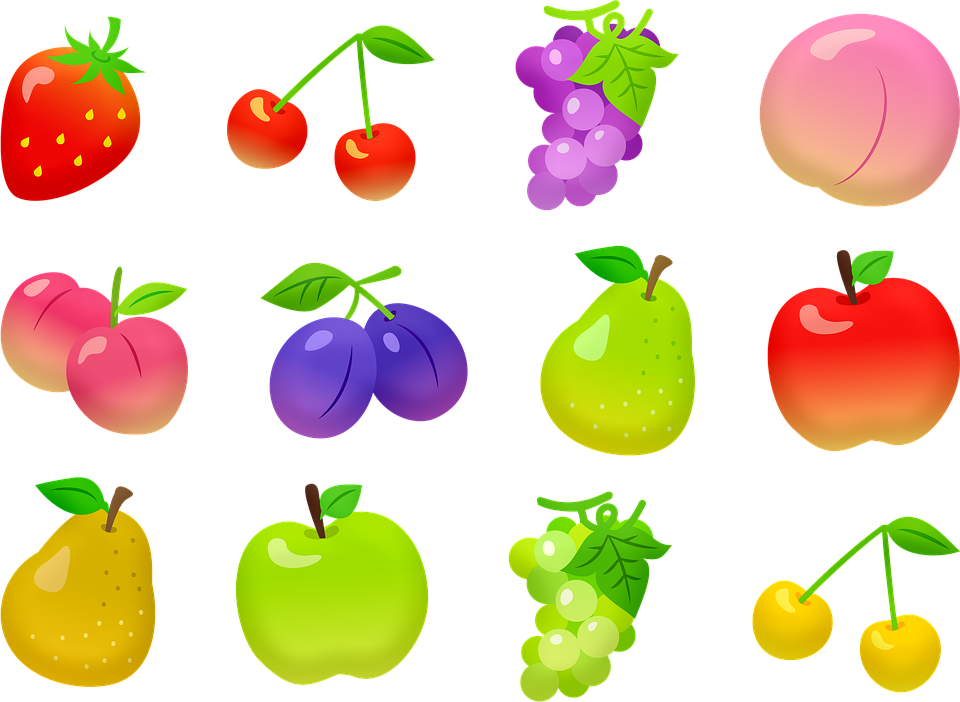
\includegraphics[trim=764 246 0 243, clip, width = 0.9cm]{02 - Combinatorics 101/fruits.png}};
          \node (apple2) at (1, 0)
              {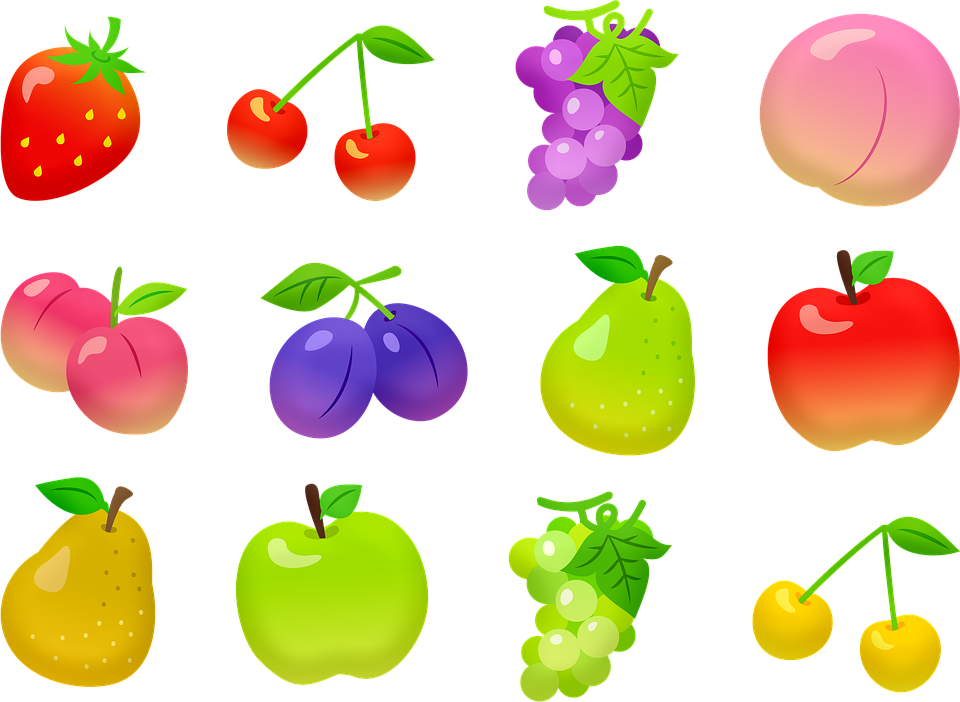
\includegraphics[trim=764 246 0 243, clip, width = 0.9cm]{02 - Combinatorics 101/fruits.png}};
          \node (apple3) at (2, 0)
              {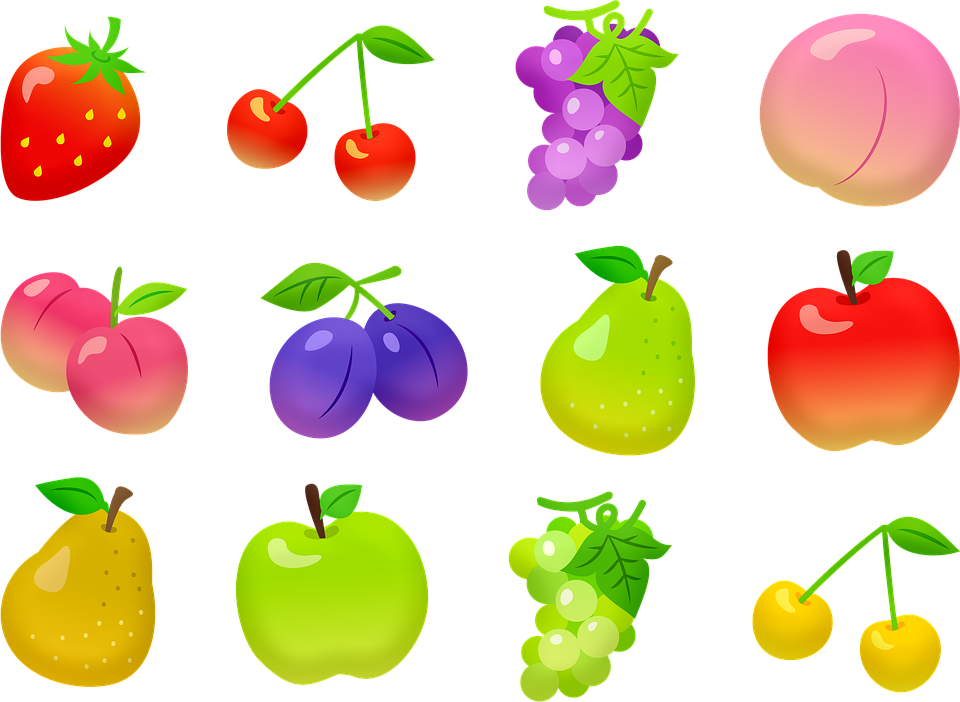
\includegraphics[trim=764 246 0 243, clip, width = 0.9cm]{02 - Combinatorics 101/fruits.png}};
          \node (pear1) at (3, 0)
              {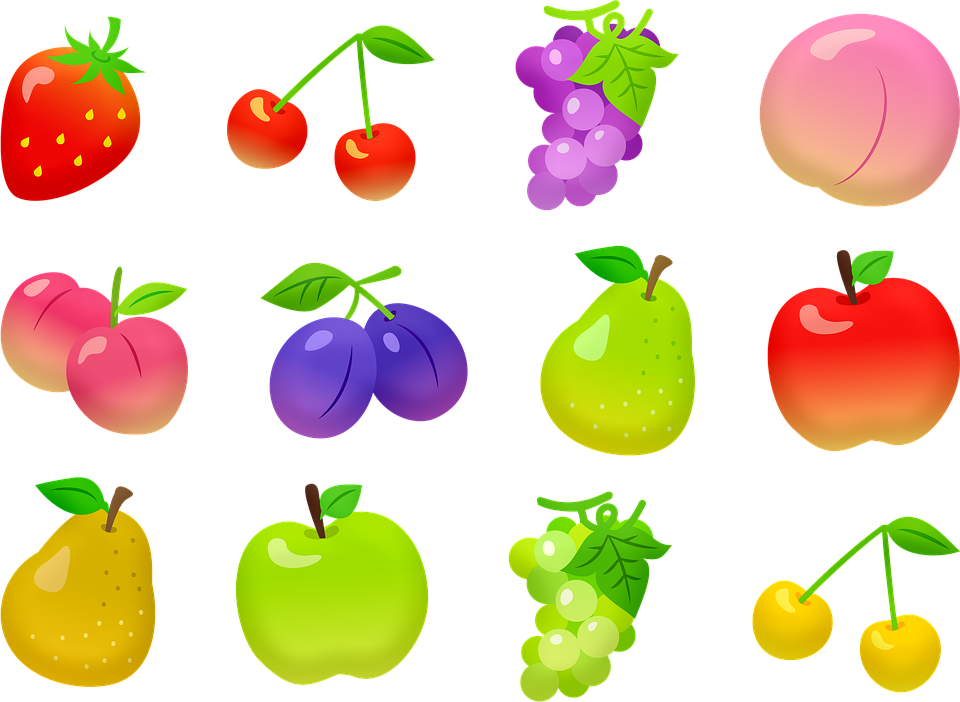
\includegraphics[trim=534 246 261 243, clip, width = 0.76cm]{02 - Combinatorics 101/fruits.png}};
          \node (pear2) at (4, 0)
              {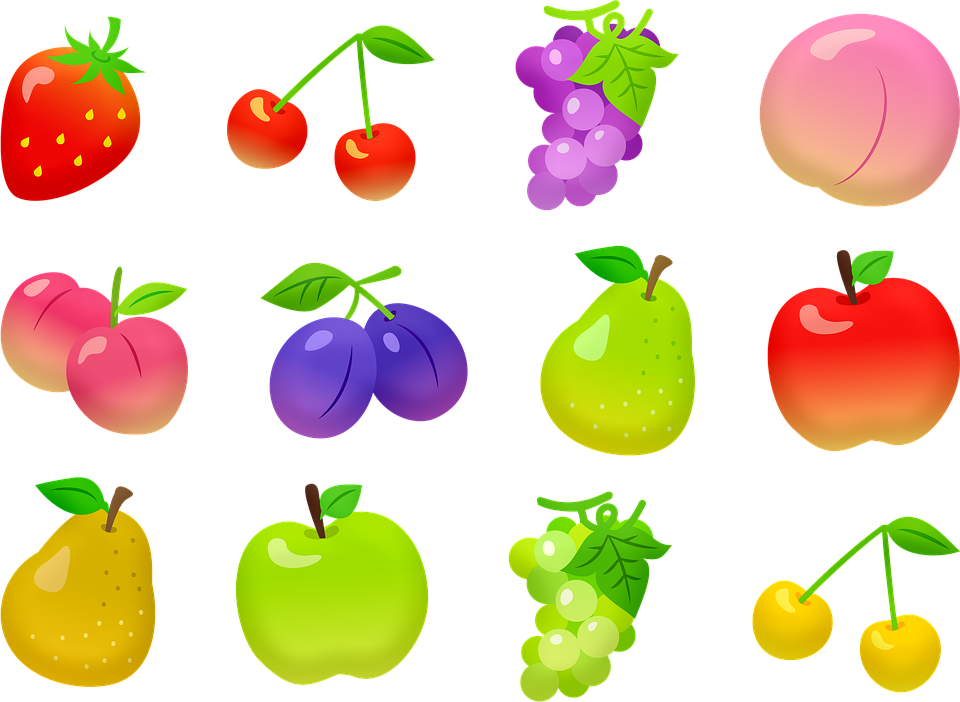
\includegraphics[trim=534 246 261 243, clip, width = 0.76cm]{02 - Combinatorics 101/fruits.png}};
        \end{tikzpicture}
      \end{nscenter}

      A solution is fairly simple. You can take one of $3$ apples or one of $2$ pears, so there are
      \[ 3 + 2 = 5 \]
      different options for you to take one fruit.
    \end{column}
    \begin{column}{0.5\textwidth}
      We have just used an operation called the \textbf{rule of sum} or \textbf{addition principle}. Stated simply, it is the intuitive idea that 

      \begin{definition}{}
        if we have $a$ number of ways of doing something and $b$ number of ways of doing another thing and we can not do both at the same time, then there are $a + b$ ways to choose one of the actions.
      \end{definition}

      Of couse this principle may be extended for many options, for example if you have $5$ plates with $10$ apples on each, there are 
      \[10+10+10+10+10 = 50\] 
      options to pick an apple.
    \end{column}
  \end{columns}
\end{frame}

\begin{frame}{Rule of product}
  \begin{columns}[T]
    \begin{column}{0.5\textwidth}
      Now we will grow a little more, and here is the problem from 3rd grade:

      \begin{problem}
        There are two plates, one with $3$ apples and one with $2$ pears. You can take \emph{one apple} and \emph{one pear}. How many options do you have?
      \end{problem}

      \begin{nscenter}
        \begin{tikzpicture}[outer sep=0, inner sep=0]
          \node (apple1) at (0, 0)
              {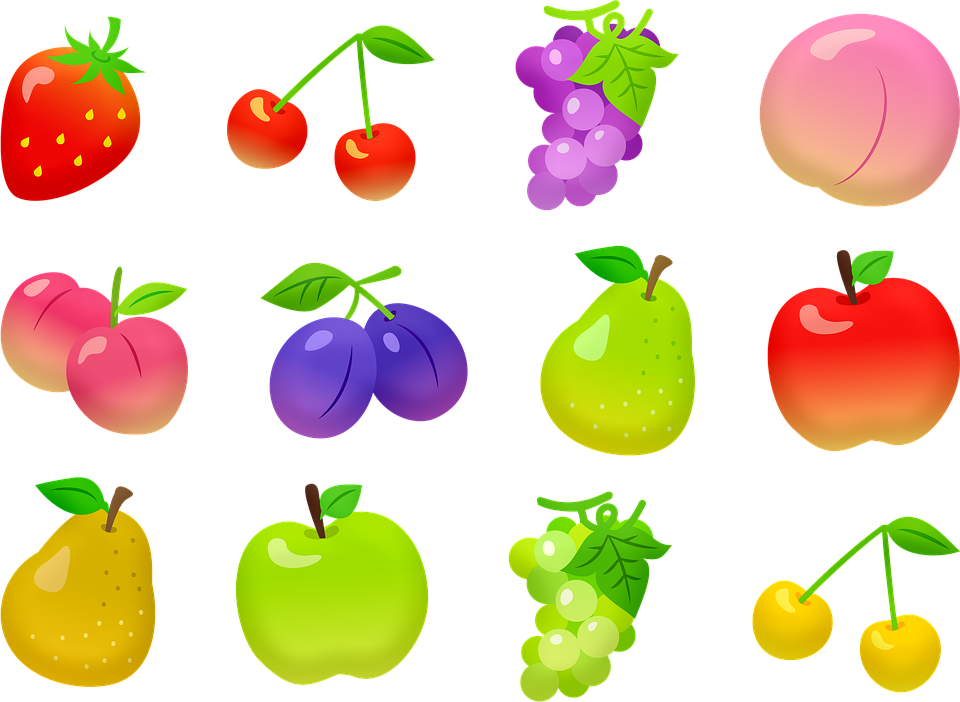
\includegraphics[trim=764 246 0 243, clip, width = 0.9cm]{02 - Combinatorics 101/fruits.png}};
          \node (apple2) at (2, 0)
              {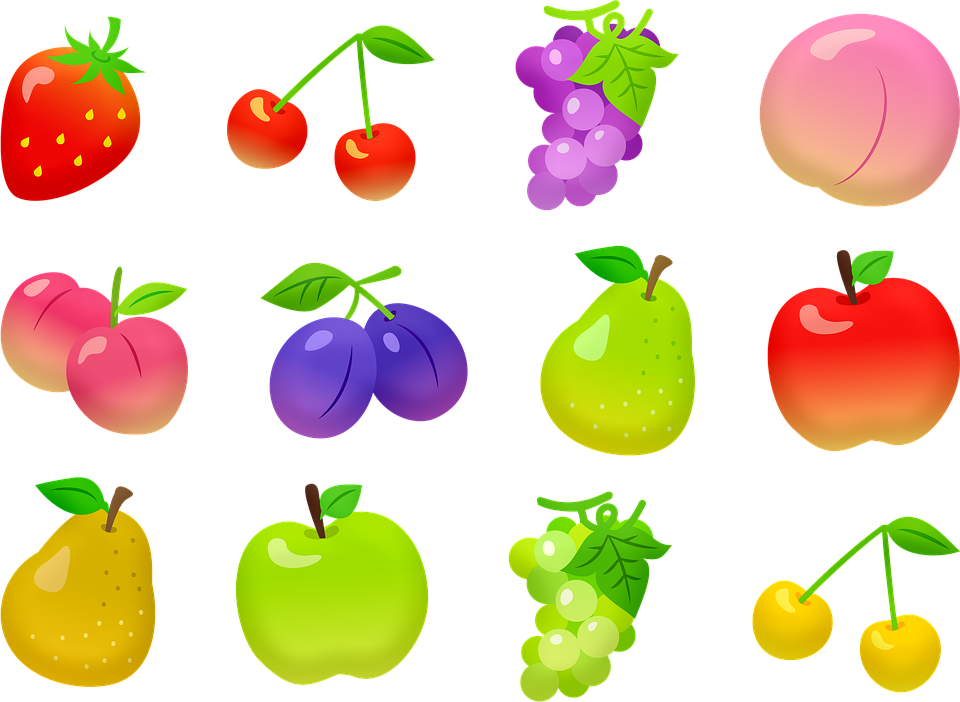
\includegraphics[trim=764 246 0 243, clip, width = 0.9cm]{02 - Combinatorics 101/fruits.png}};
          \node (apple3) at (4, 0)
              {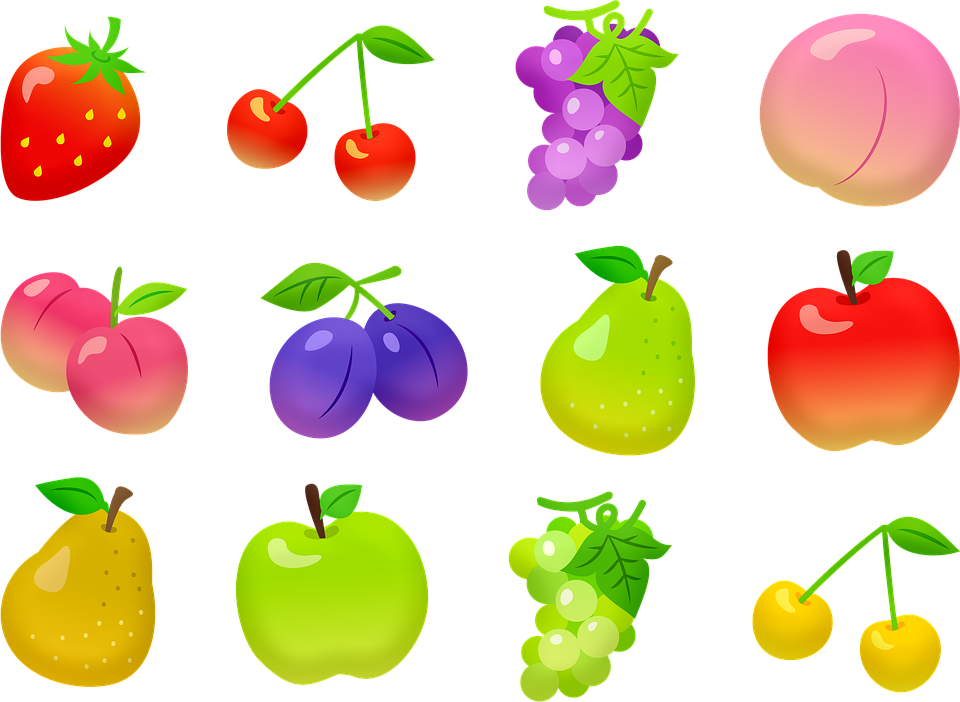
\includegraphics[trim=764 246 0 243, clip, width = 0.9cm]{02 - Combinatorics 101/fruits.png}};
          \node (pear1) at (1, -0.33)
              {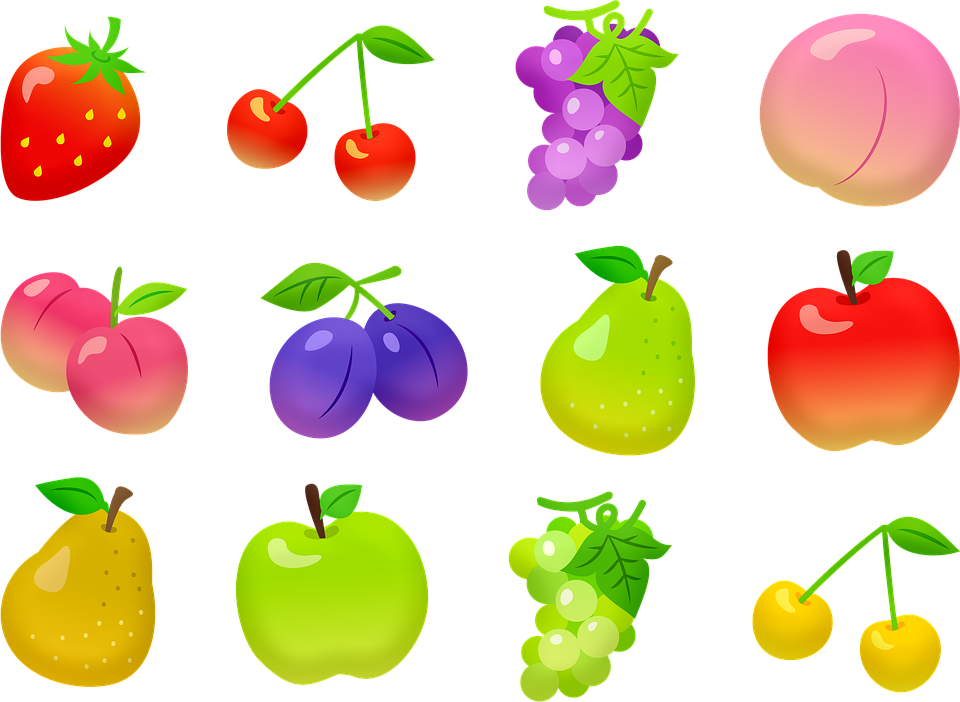
\includegraphics[trim=534 246 261 243, clip, width = 0.76cm]{02 - Combinatorics 101/fruits.png}};
          \node (pear2) at (3, -0.33)
              {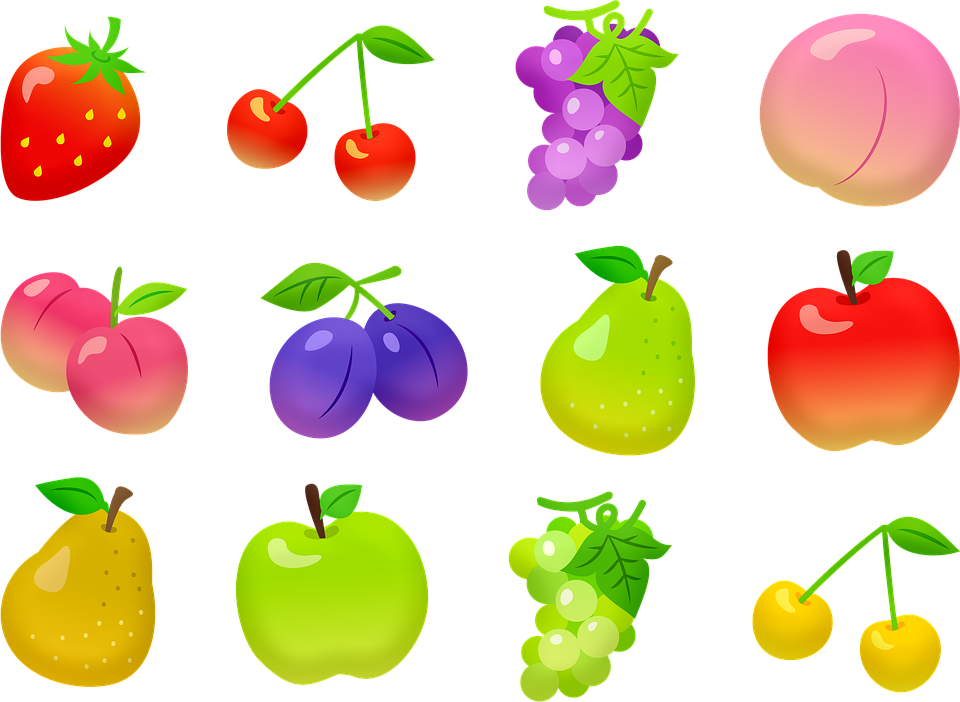
\includegraphics[trim=534 246 261 243, clip, width = 0.76cm]{02 - Combinatorics 101/fruits.png}};
        \end{tikzpicture}
      \end{nscenter}

      A solution is also not that hard. You can take one of $3$ apples, so you have $3$ options for the first choice, then for each choice, you have $2$ options to select one pear. So you have 
      \[3 \times 2 = 6\] 
      different options for you to take one apple and one pear.

    \end{column}
    \begin{column}{0.5\textwidth}
      We've just used the \textbf{rule of product} or \textbf{multiplication principle}. Stated simply, it is the idea that 
      \begin{definition}
        if there are $a$ ways of doing something and $b$ ways of doing another thing, then there are $a \times b$ ways of performing both actions.
      \end{definition}

      Of course, this principle may be extended for many options, for example if you have $5$~plates with $10$ apples on each, there are
      \[ 10 \times 10 \times 10 \times 10 \times 10 = 100,000 \]
      options to pick one apple from each plate.

      \vspace*{1em}

      \begin{example}
        Both the \emph{rule of sum} and the \emph{rule of product} are called \emph{\textbf{basic counting principles}}.
      \end{example}
    \end{column}
  \end{columns}
\end{frame}

\begin{frame}{Permutations}
  \begin{columns}[T]
    \begin{column}{0.5\textwidth}
      Now move to a problem worth 5th-grade.
      \begin{problem}
        There are $5$ different fruits on a plate: \emph{a red apple}, \emph{a pear}, \emph{a strawberry}, \emph{a peach}, and \emph{a~green apple}. You have to take \textbf{all of them} \emph{one by one}. In how many ways can you do that?
      \end{problem}

      \begin{nscenter}
        \begin{tikzpicture}[outer sep=0, inner sep=0, scale=1, transform shape]
          \node (apple1) at (0, 0)
              {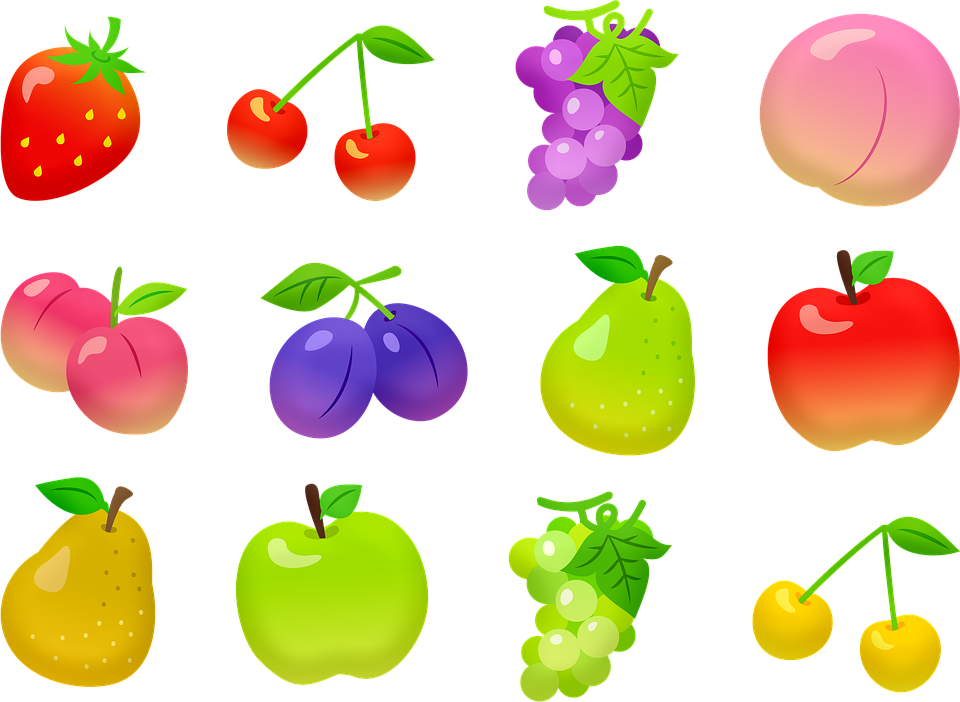
\includegraphics[trim=764 246 0 243, clip, width = 0.9cm]{02 - Combinatorics 101/fruits.png}};
          \node (pear1) at (1, 0)
              {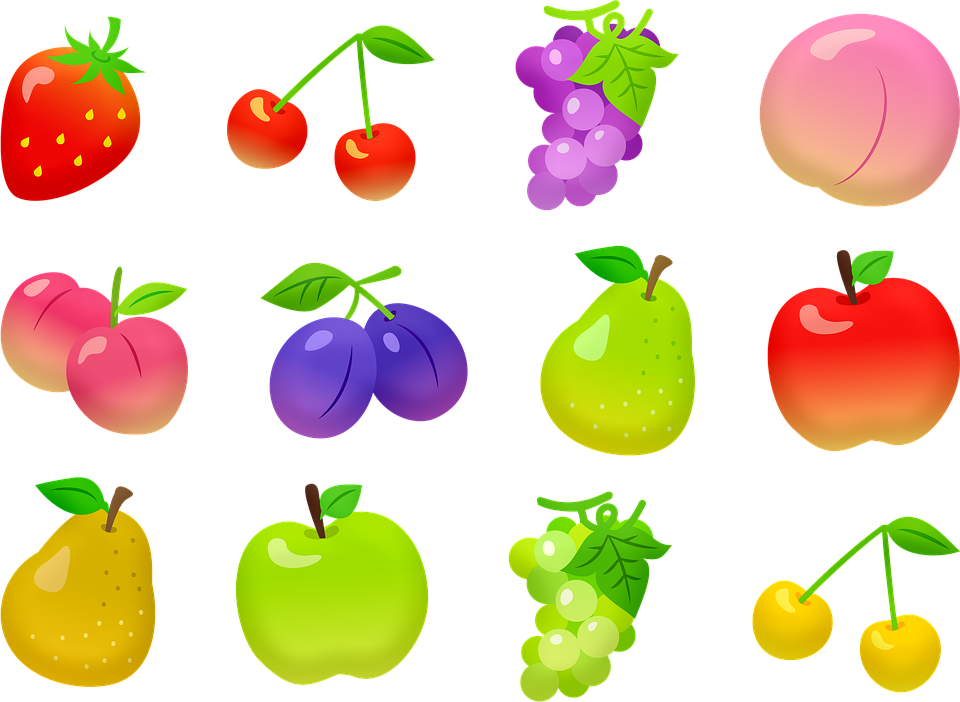
\includegraphics[trim=534 246 261 243, clip, width = 0.76cm]{02 - Combinatorics 101/fruits.png}};
          \node (strawberry1) at (1.95, 0)
              {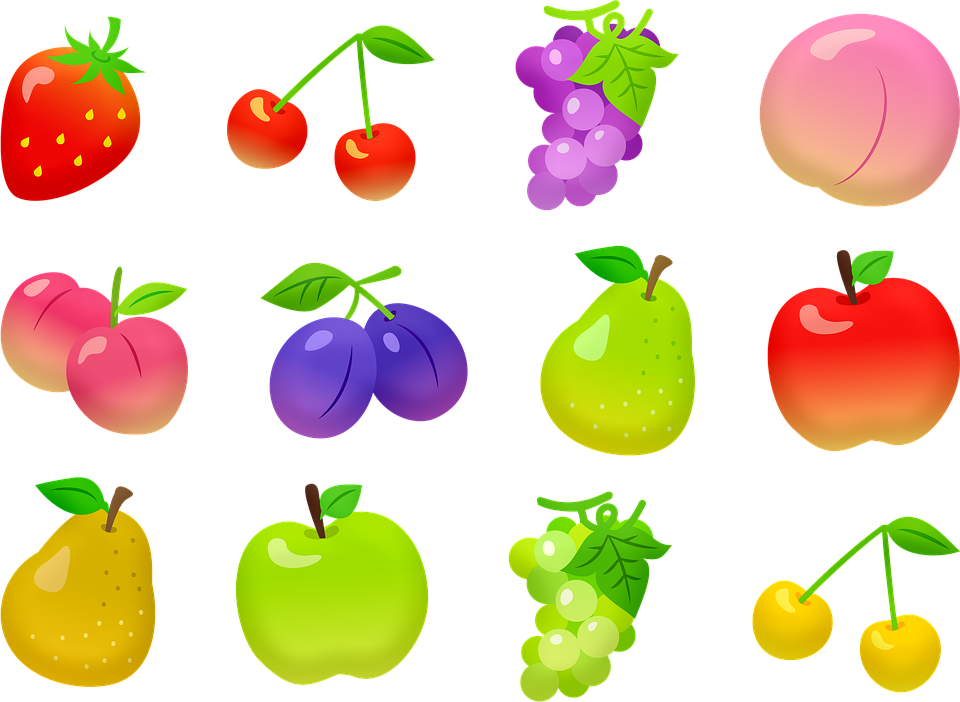
\includegraphics[trim=0 490 809 0, clip, width = 0.69cm]{02 - Combinatorics 101/fruits.png}};
          \node (peach1) at (2.9, 0)
              {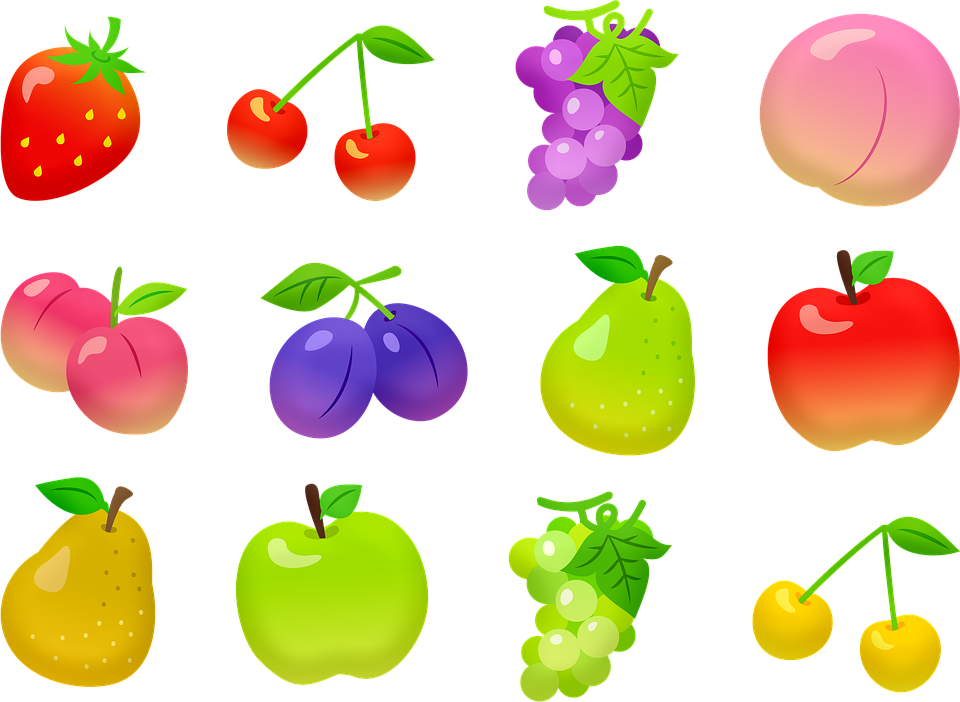
\includegraphics[trim=751 491 0 0, clip, width = 0.96cm]{02 - Combinatorics 101/fruits.png}};
          \node (apple2) at (4, 0)
              {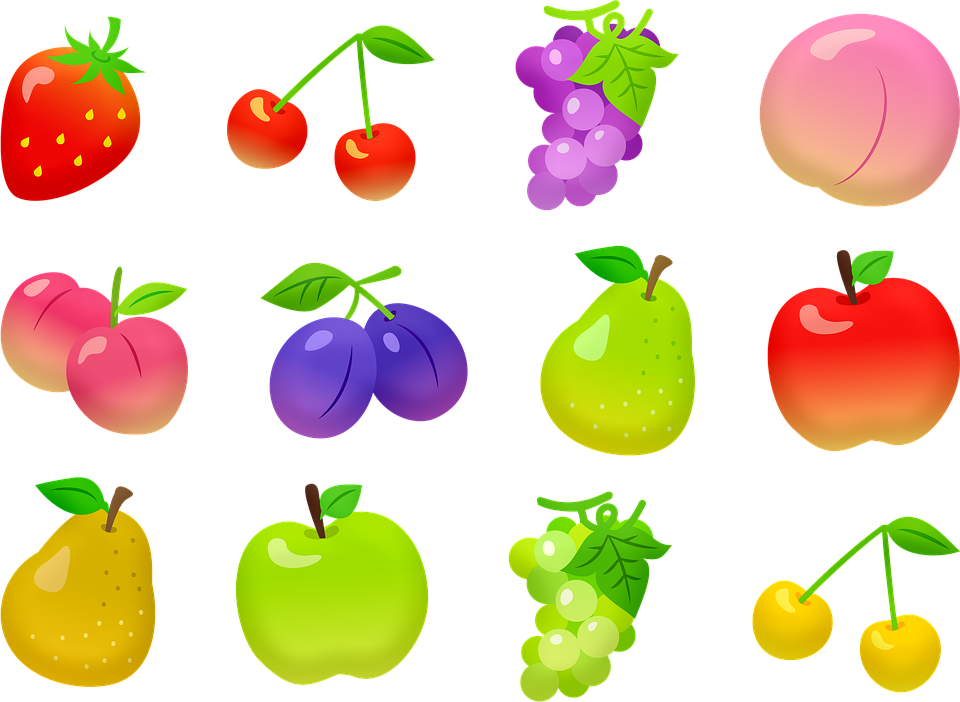
\includegraphics[trim=232 0 532 472, clip, width = 0.9cm]{02 - Combinatorics 101/fruits.png}};
        \end{tikzpicture}
      \end{nscenter}

      The first fruit can be any of these, so we have $5$ options to take it. 

      There are $4$ fruits left, and now we have $4$ options. 
      
      Then $3$ fruit left and we have $3$ options. 
      
      For $2$ leftover fruits, we have only $2$ options and for the last fruit, we have only $1$ option to choose from.

      By the \textbf{rule of product}, there are
      \[5 \times 4 \times 3 \times 2 \times 1 = 120\]
      ways to pick $5$ fruits one by one. 
    \end{column}
    \begin{column}{0.5\textwidth}
      In combinatorics, 
      \begin{definition}
        a \textbf{permutation} is an ordering of a list of objects.
      \end{definition}
      To find a number of permutations of $n$ distinct objects (denoted as $P_n$), we need, according to the \emph{rule of product}, to multiply the following numbers: $n \times (n − 1) \times (n − 2) \times \ldots \times 2 \times 1$.
      This product is called the \textbf{factorial} and denoted by $n!$. So for any positive integer $n$,
      \begin{definition}
        \centering $n! = 1 \times 2 \times \ldots \times (n − 1) \times n,$
      \end{definition} 
      In words:
      \begin{example}
        $n!$ is the product of all positive integers from $1$ to~$n$.
      \end{example}

      We also define $0! = 1$, because there is one permutation of the empty list of objects. It is the empty permutation. 
    \end{column}
  \end{columns}
\end{frame}

\begin{frame}{Rule of division}
  \begin{columns}[T]
    \begin{column}{0.5\textwidth}
      Let's simplify the previous problem.
      \begin{problem}
        There are $5$ different fruits on a plate: \emph{a red apple}, \emph{a pear}, \emph{a strawberry}, \emph{a peach}, and \emph{a green apple}. You have to \textbf{take $3$ of them} all \emph{one by one}. In how many ways can you do that?
      \end{problem}

      \begin{nscenter}
        \begin{tikzpicture}[outer sep=0, inner sep=0, scale=1, transform shape]
          \node (apple1) at (0, 0)
              {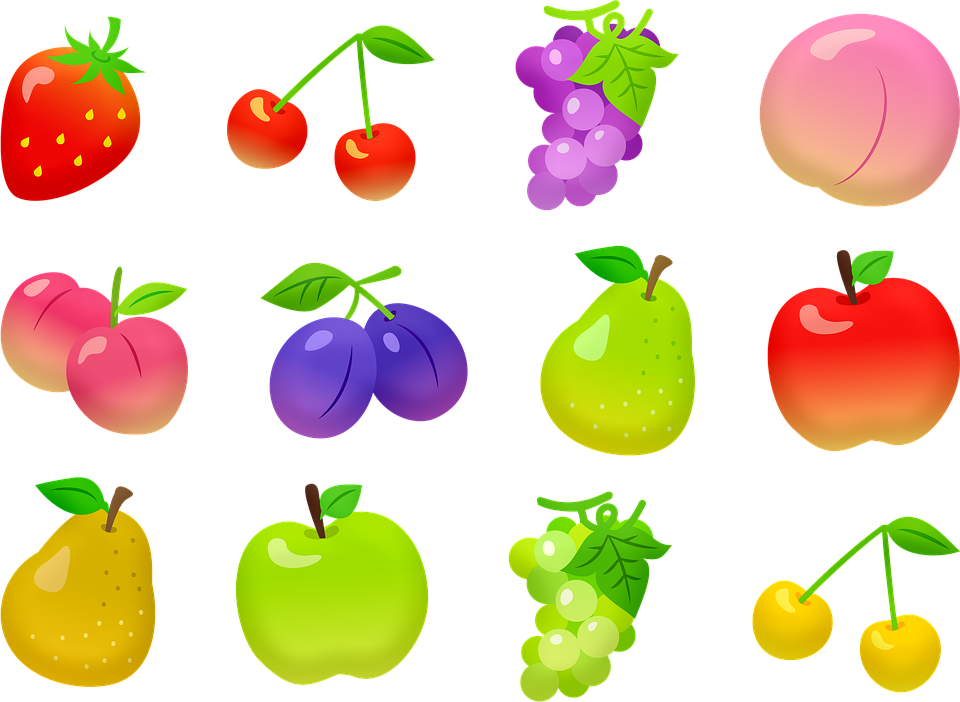
\includegraphics[trim=764 246 0 243, clip, width = 0.9cm]{02 - Combinatorics 101/fruits.png}};
          \node (pear1) at (1, 0)
              {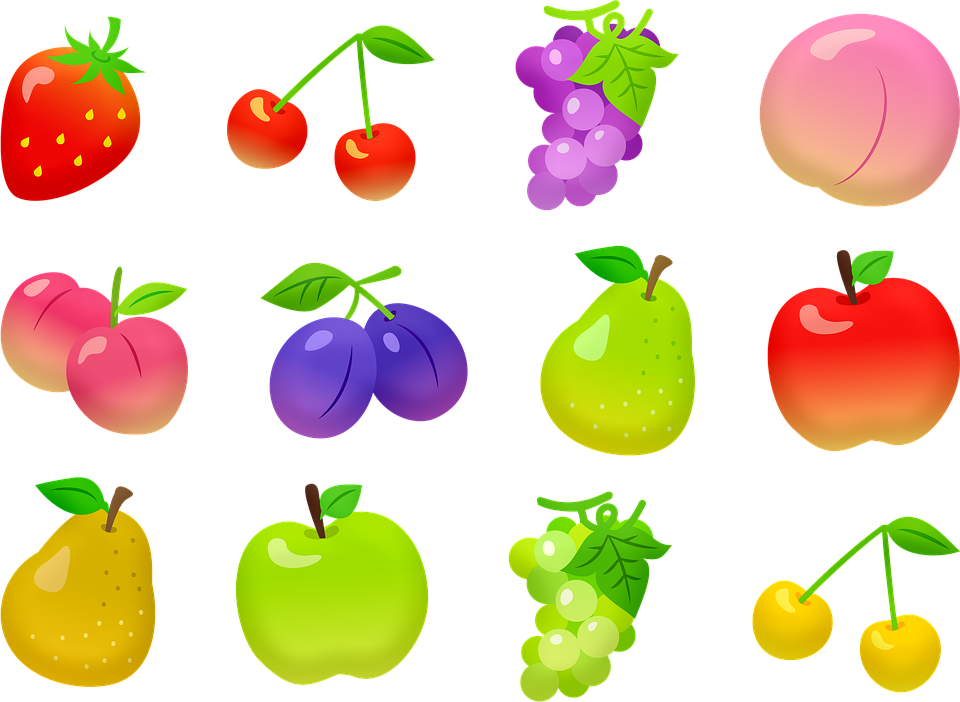
\includegraphics[trim=534 246 261 243, clip, width = 0.76cm]{02 - Combinatorics 101/fruits.png}};
          \node (strawberry1) at (1.95, 0)
              {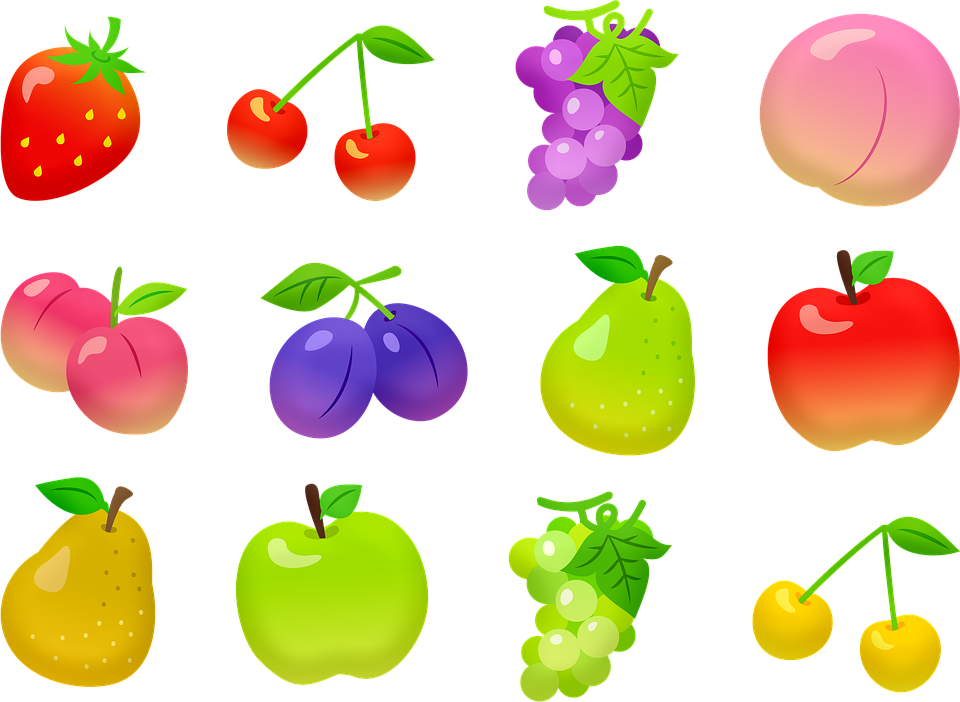
\includegraphics[trim=0 490 809 0, clip, width = 0.69cm]{02 - Combinatorics 101/fruits.png}};
          \node[opacity=.3] (peach1) at (2.9, 0)
              {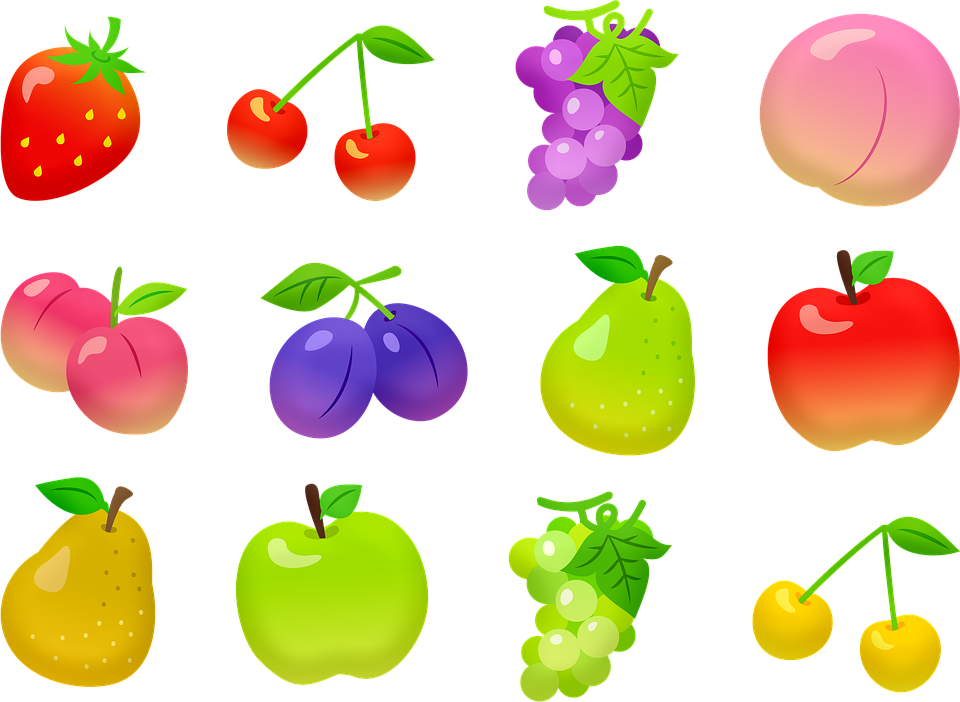
\includegraphics[trim=751 491 0 0, clip, width = 0.96cm]{02 - Combinatorics 101/fruits.png}};
          \node[opacity=.3] (apple2) at (4, 0)
              {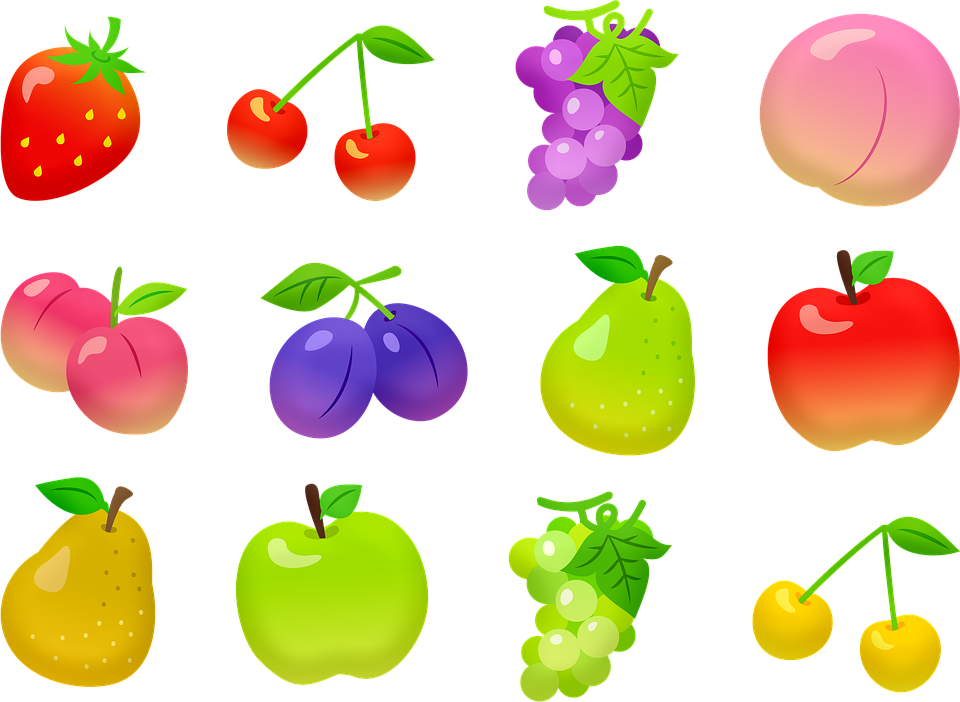
\includegraphics[trim=232 0 532 472, clip, width = 0.9cm]{02 - Combinatorics 101/fruits.png}};
        \end{tikzpicture}
      \end{nscenter}

      The solution would be similar to the previous one, except we will stop on $3$rd step. So there are
      \[5 \times 4 \times 3 = 60\] 
      ways to pick $3$ fruits one by one. 

      Another way to think about the solution, that considers all the way to pick two remaining fruits as one option. So we will get the same result by the following operation:
      \[
        \frac{5 \times 4 \times 3 \times 2 \times 1 \text{\ total number of ways}}{2 \times 1 \text{\  ways to get remainder}} = \frac{5!}{2!} = 60.
      \]
    \end{column}
    \begin{column}{0.5\textwidth}
      The second approach use the \textbf{rule of division}:
      \begin{definition}
        if \emph{some} options are considered the same, we can \textbf{divide} the \emph{total number} of options by the \emph{number of options} we considered the same.
      \end{definition}

      So if we have $n$ objects and want to arrange $k$ of them in a row, there are $\frac{n!}{(n-k)!}$ ways to do this. This is also known as a $k$-permutation of $n$, and is denoted by $P_k^n$ or $P(n,\ k)$.\medskip

      The rule of division is also works in case when we need to put $5$ fruits not in a line, but in a circle. In this case this $5$ permutations are the same:
      \vspace*{-0.1cm}
      \begin{nscenter}
        \begin{tikzpicture}[outer sep=0, inner sep=0]
          \node (plate1) at (0, 0)
              {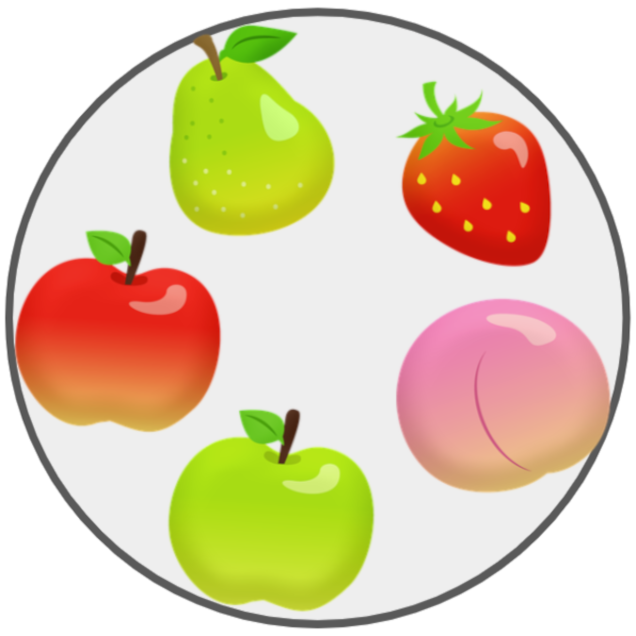
\includegraphics[width = 1.2cm]{02 - Combinatorics 101/plate.png}};
          \node[rotate=-72] (plate2) at (1.3, 0)
              {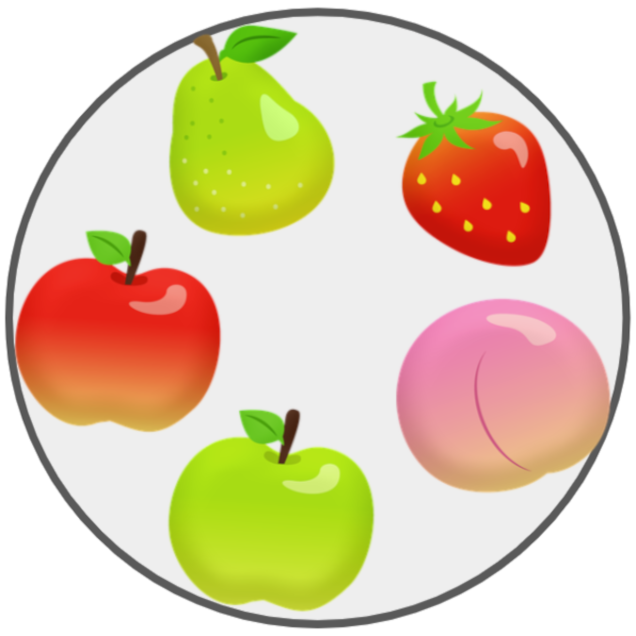
\includegraphics[width = 1.2cm]{02 - Combinatorics 101/plate.png}};
          \node[rotate=-144] (plate3) at (2.6, 0)
              {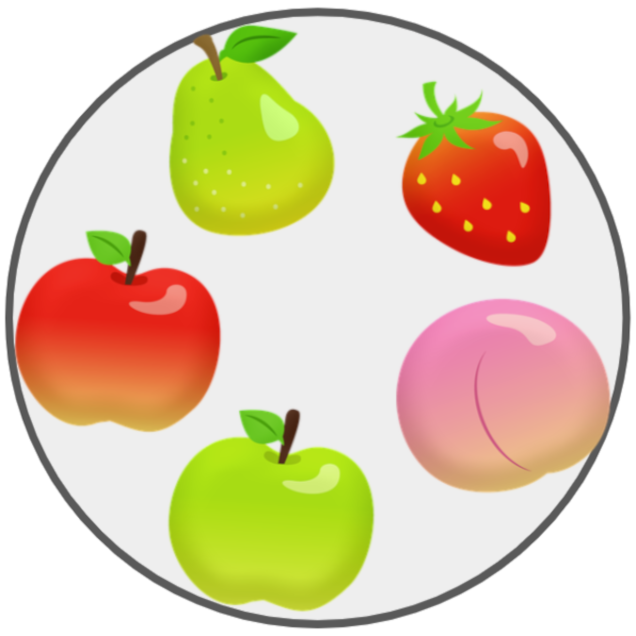
\includegraphics[width = 1.2cm]{02 - Combinatorics 101/plate.png}};
          \node[rotate=-216] (plate4) at (3.9, 0)
              {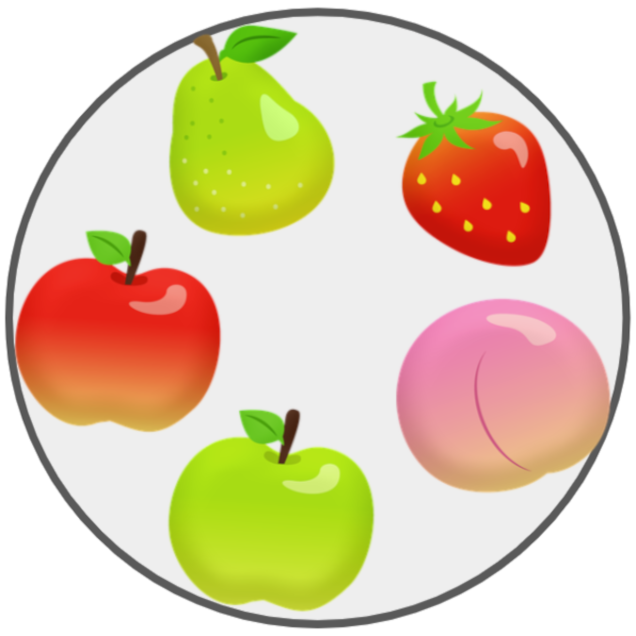
\includegraphics[width = 1.2cm]{02 - Combinatorics 101/plate.png}};
          \node[rotate=-288] (plate5) at (5.2, 0)
              {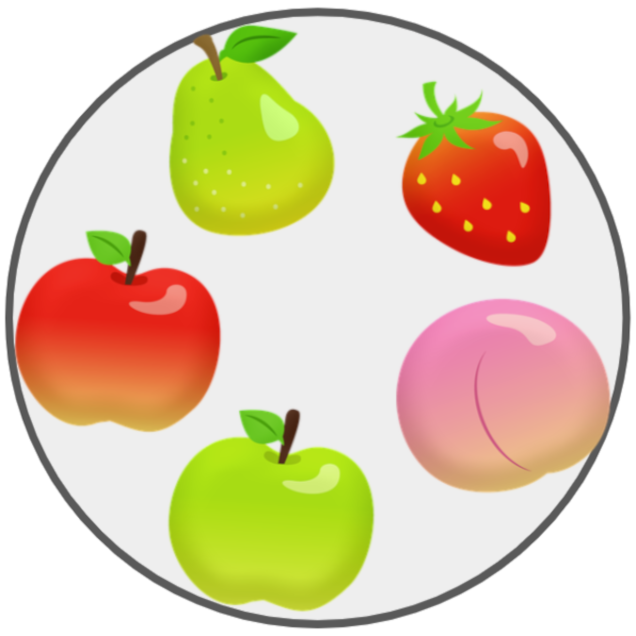
\includegraphics[width = 1.2cm]{02 - Combinatorics 101/plate.png}};
        \end{tikzpicture}
      \end{nscenter}
      \vspace*{-0.2cm}
      so the total number of ways to put of $5$ elements in a circle is $\frac{5!}{5} = 24$.
    \end{column}
  \end{columns}
\end{frame}

\begin{frame}{Permutations with identical elements}
  \begin{columns}[T]
    \begin{column}{0.5\textwidth}
      Now get back to problem from Kindergarten

      \begin{problem}
        There is a plate with $3$ apples and with $1$ pear and $1$ strawberry. In how many ways can you take all of the pieces of fruit \emph{one by one}, if all apples are considered the same?
      \end{problem}

      \begin{nscenter}
        \begin{tikzpicture}[outer sep=0, inner sep=0]
          \node (apple1) at (0, 0)
              {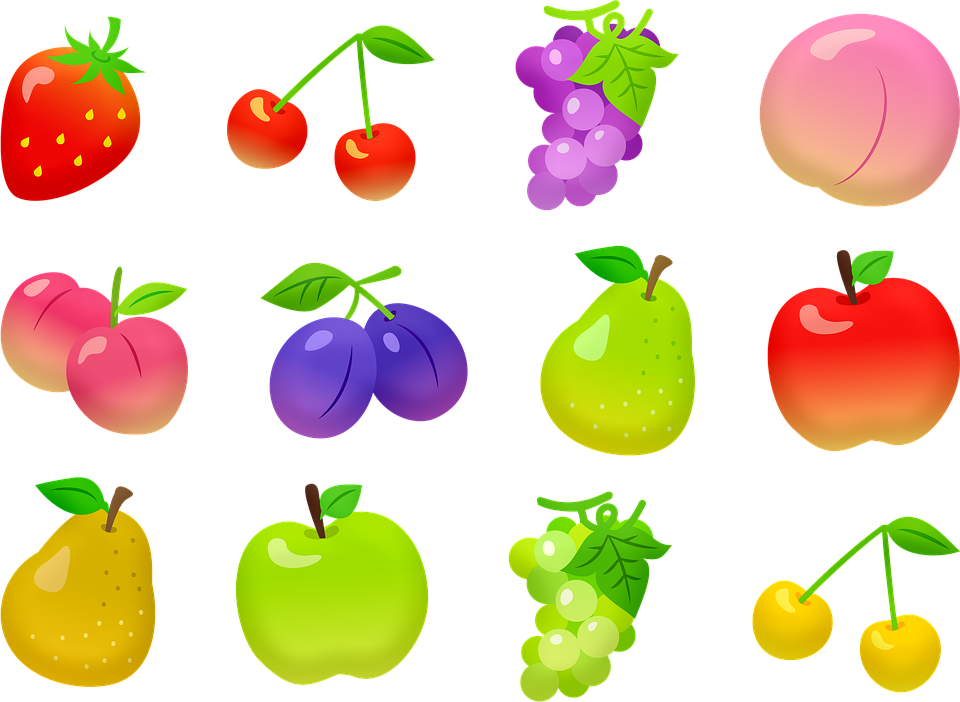
\includegraphics[trim=764 246 0 243, clip, width = 0.9cm]{02 - Combinatorics 101/fruits.png}};
          \node (apple2) at (1, 0)
              {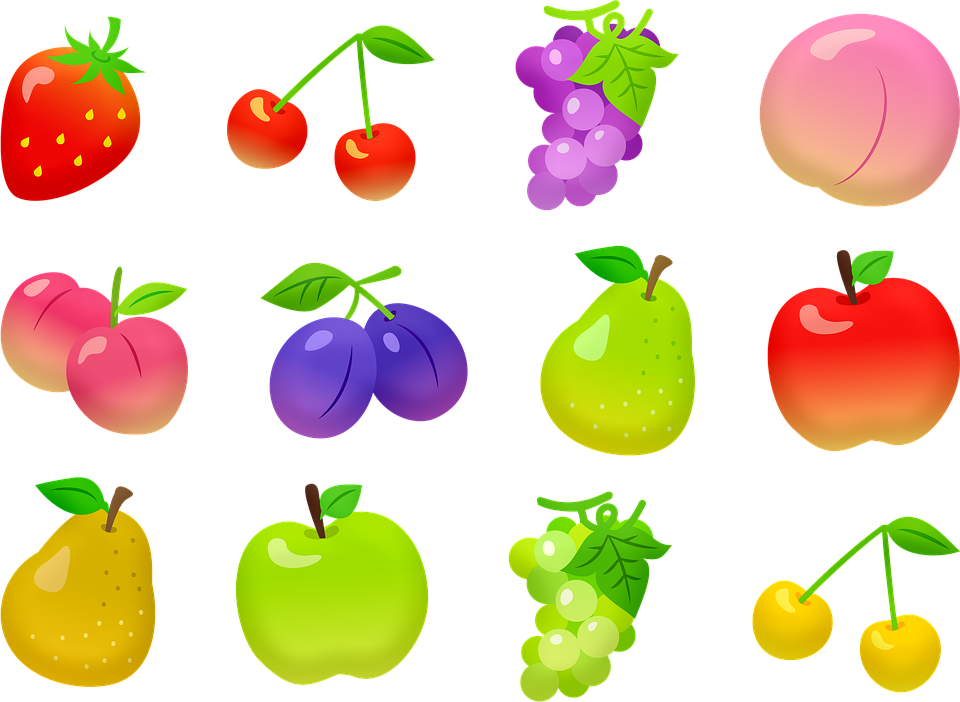
\includegraphics[trim=764 246 0 243, clip, width = 0.9cm]{02 - Combinatorics 101/fruits.png}};
          \node (apple3) at (2, 0)
              {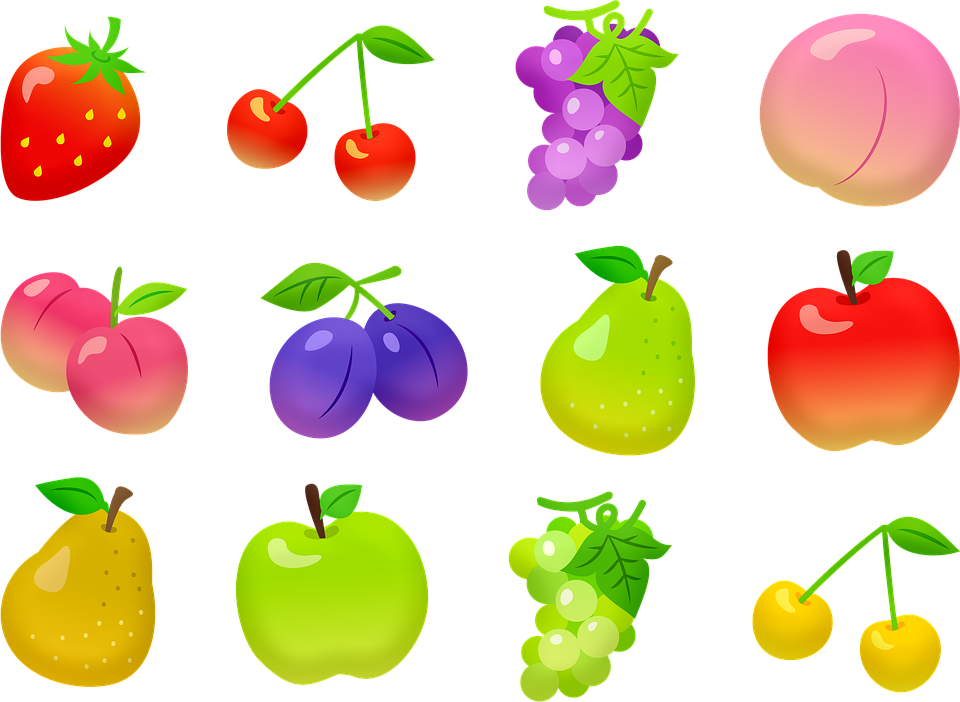
\includegraphics[trim=764 246 0 243, clip, width = 0.9cm]{02 - Combinatorics 101/fruits.png}};
          \node (pear1) at (3, 0)
              {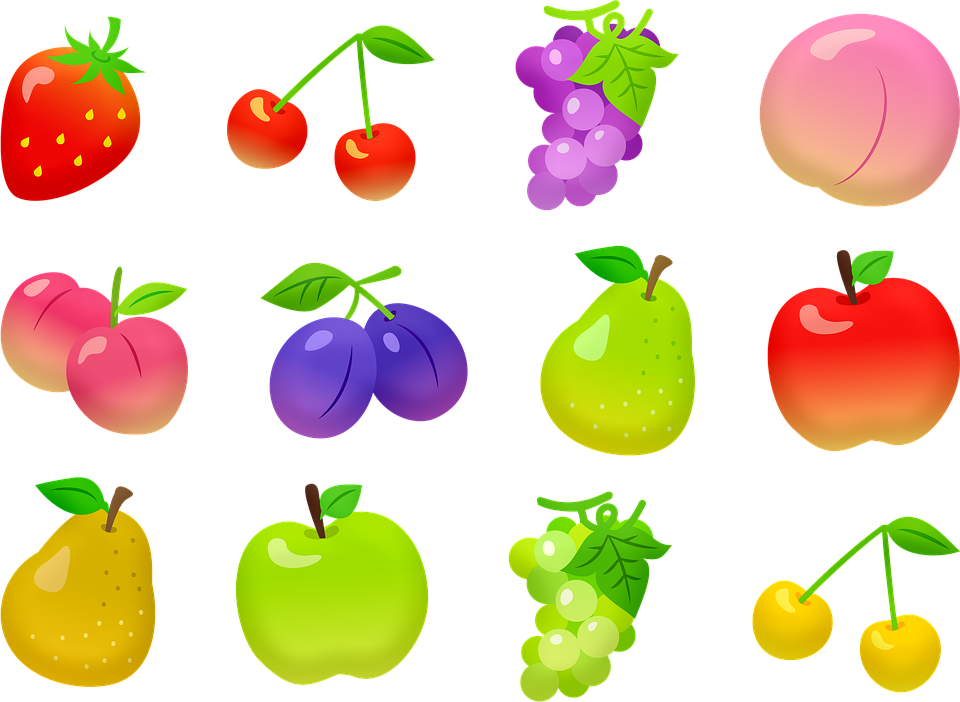
\includegraphics[trim=534 246 261 243, clip, width = 0.76cm]{02 - Combinatorics 101/fruits.png}};
          \node (strawberry1) at (4, 0)
              {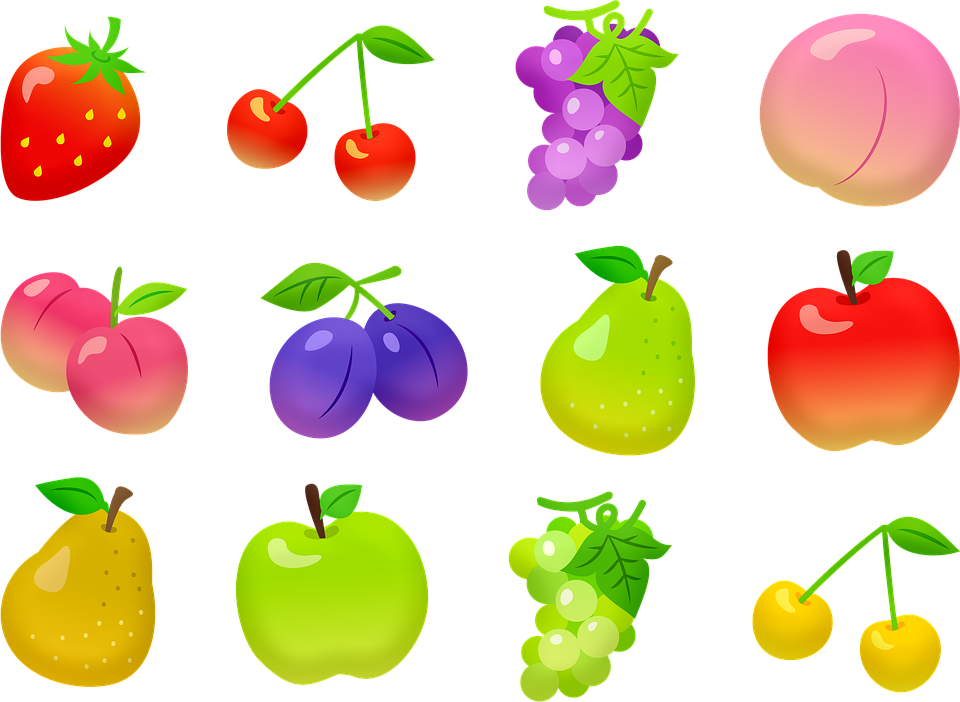
\includegraphics[trim=0 490 809 0, clip, width = 0.69cm]{02 - Combinatorics 101/fruits.png}};
        \end{tikzpicture}
      \end{nscenter}

      {\small
      We already know, that there are $5! = 120$ total orders if all apples are different. But consider the options,when apples are at places $1$, $2$, and $3$. There are a total $3! = 6$ cases when we can put apples in these places. That means for every order, there are $5$ other orders that are the same when all apples are the same, because we can’t distinguish the $6$ ways we can arrange apples from one another. So total number of permutations is}
      \[
        \frac{5!}{3!} = \frac{120}{6} = 20.
      \]
    \end{column}
    \begin{column}{0.5\textwidth}
      \begin{problem}
        There is a plate with $3$ apples and $2$ strawberries. In how many ways can you take all of the fruit \emph{one by one}, if selections of each type of fruit are the same?
      \end{problem}

      \begin{nscenter}
        \begin{tikzpicture}[outer sep=0, inner sep=0, scale=0.8, transform shape]
          \node (apple1) at (0, 0)
              {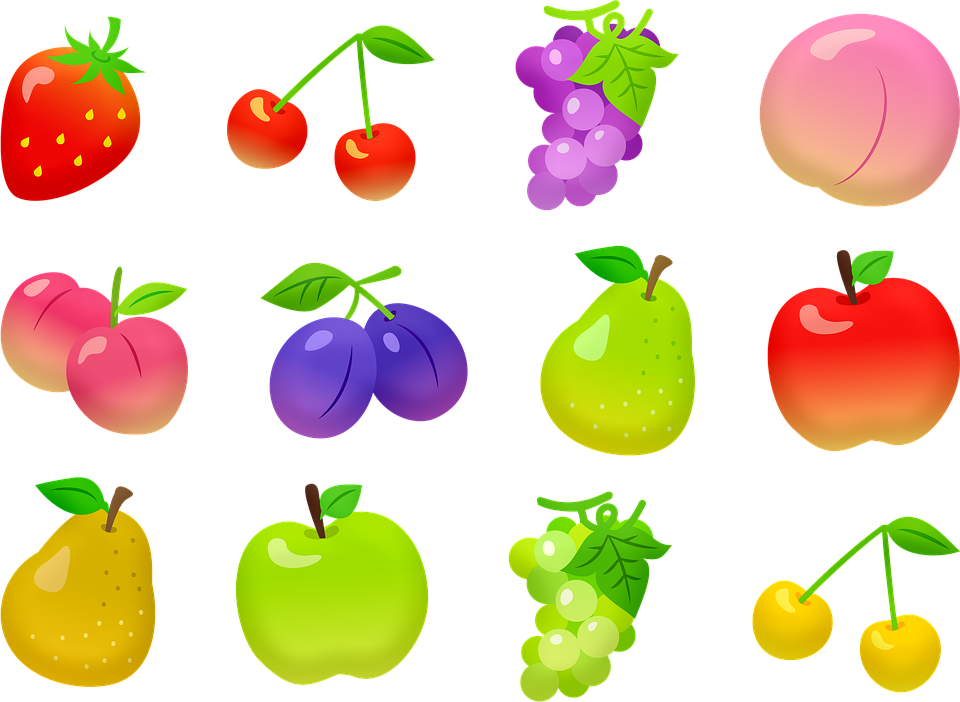
\includegraphics[trim=764 246 0 243, clip, width = 0.9cm]{02 - Combinatorics 101/fruits.png}};
          \node (apple2) at (1, 0)
              {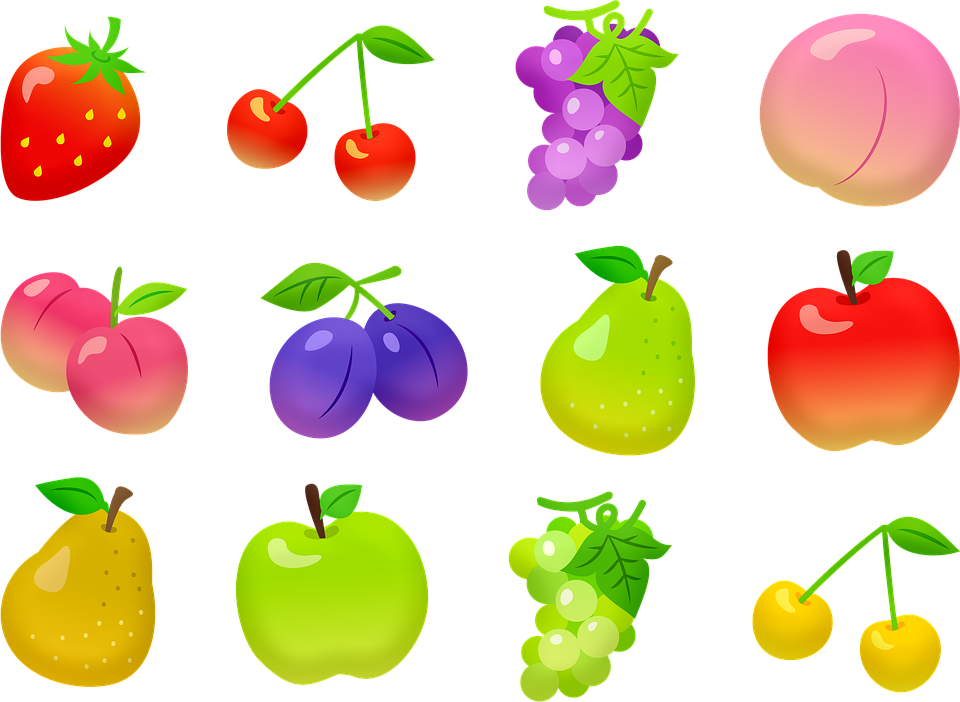
\includegraphics[trim=764 246 0 243, clip, width = 0.9cm]{02 - Combinatorics 101/fruits.png}};
          \node (apple3) at (2, 0)
              {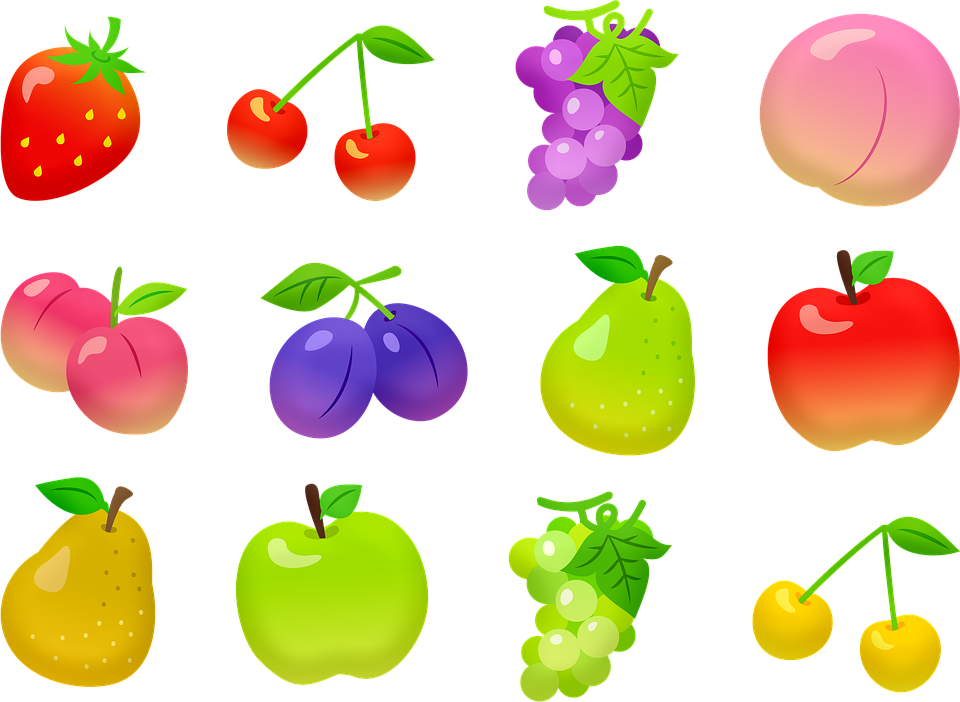
\includegraphics[trim=764 246 0 243, clip, width = 0.9cm]{02 - Combinatorics 101/fruits.png}};
          \node (strawberry1) at (3, 0)
              {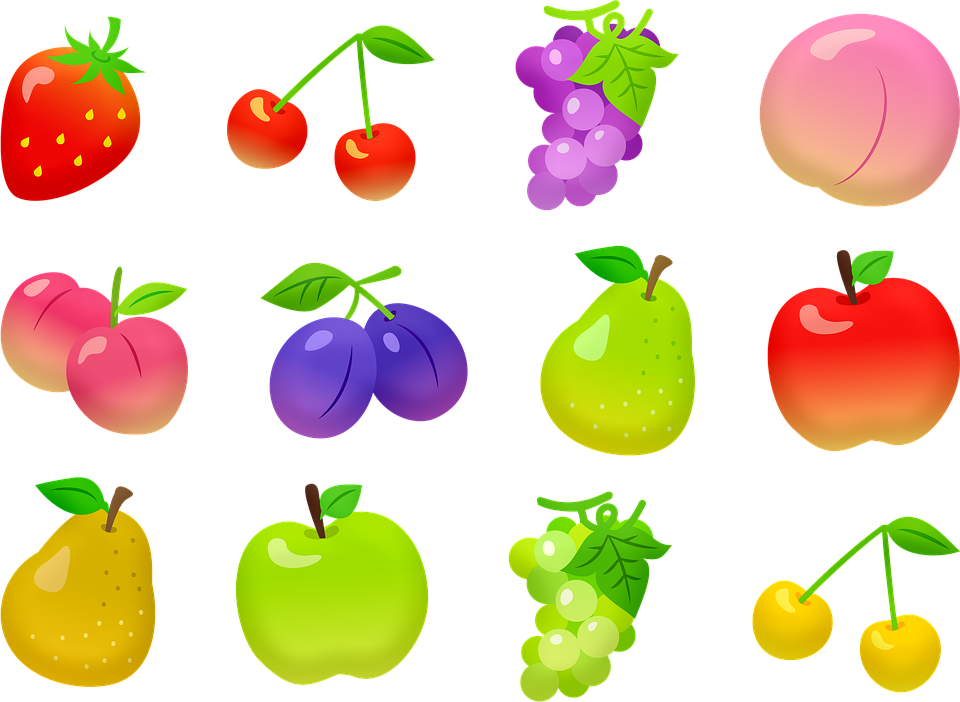
\includegraphics[trim=0 490 809 0, clip, width = 0.69cm]{02 - Combinatorics 101/fruits.png}};
          \node (strawberry2) at (4, 0)
              {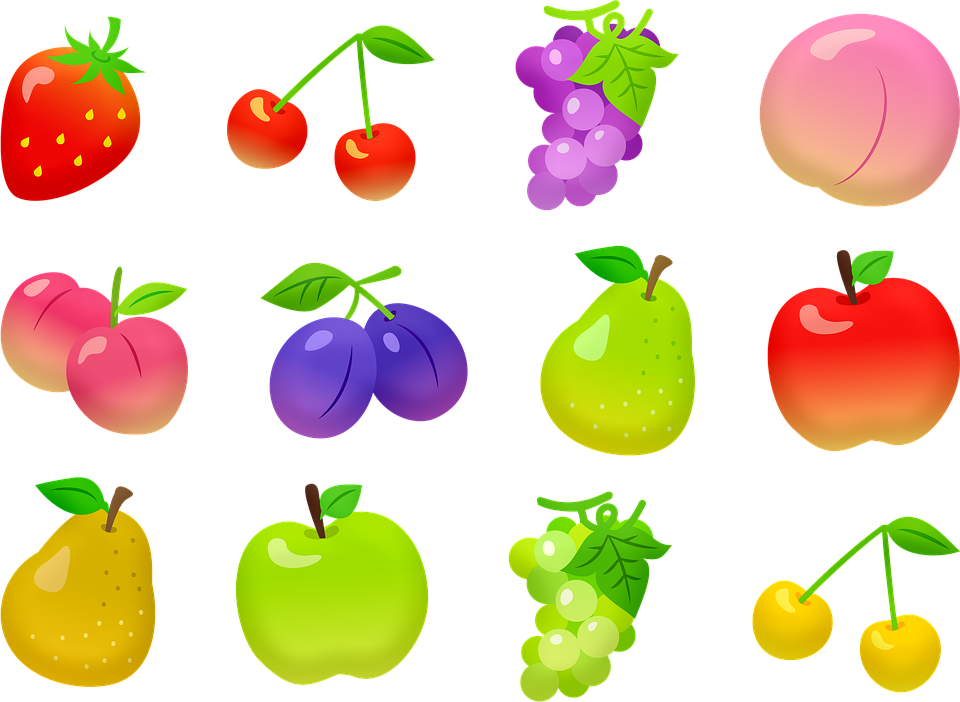
\includegraphics[trim=0 490 809 0, clip, width = 0.69cm]{02 - Combinatorics 101/fruits.png}};
        \end{tikzpicture}
      \end{nscenter}

      {\small
      We already know, that there are $5! = 120$ total orders if all apples and strawberries are different. We just saw that there are $3!$ identical arrangements of apples. In addition, we now have $2!$ identical arrangements of strawberries.  So the total number of permutations is:
      \[
        \frac{5!}{3! \times 2!} = \frac{120}{12} = 10.
      \]}

      \begin{definition}
        In general, if there are total $N$ objects, and $n_a$, $n_b$, $n_c$, $\dots$ are the number of copies of the same objects, then there are 
        $
          \frac{N!}{n_a! n_b! n_c!\ \ldots}
        $
        permutations in the set.
      \end{definition}
    \end{column}
  \end{columns}
\end{frame}

\begin{frame}{Permutations with restrictions}
  \begin{columns}[T]
    \begin{column}{0.5\textwidth}
      Sometimes additional restrictions may be imposed in a problem. Consider this problem
      \begin{problem}
        There are $3$ algebra books and $2$ geometry books. In how many ways can you put them on a shelf, so given \emph{subject books are kept together}?        
      \end{problem}
      \begin{wrapfigure}{r}{0.3\textwidth}\centering
        
\includegraphics[width=0.3\textwidth]{02 - Combinatorics 101/books.png}
      \end{wrapfigure}

      First we need to decide which subject will go first. There are $2!$ options for that. Then we need to decide an order of algebra books, we have $3!$ options. Similarly, for geometry books there are $2!$ options. So total number of ways is
      \[
        2! \times 3! \times 2! = 2 \times 6 \times 2 = 24.
      \]
    \end{column}
    \begin{column}{0.5\textwidth}
      When additional restrictions are imposed, the situation is transformed into a problem about \textbf{permutations with restrictions}.\medskip

      Most commonly, the restriction is that only a small number of objects are to be considered, meaning that not all the objects need to be ordered. Other common types of restrictions include restricting the type of objects that can be adjacent to one another, or changing the ordering mechanism from a line to another configuration (e.g. a round table instead of a line, or a keychain instead of a ring).\medskip

      Problems of this form are perhaps the most common in practice.

    \end{column}
  \end{columns}
\end{frame}

\begin{frame}{Permutations in problems}
  \begin{columns}[T]
    \begin{column}{0.5\textwidth}
      Now instead of a plate we have unlimited supply of fruits
      \begin{problem}
        There is $4$ bags with fruits: \emph{apples}, \emph{pears}, \emph{peaches} and \emph{strawberries}? You need to pick $5$ fruits \emph{one by one}. In how may way you can do it?
      \end{problem}

      \begin{nscenter}
        \begin{tikzpicture}[outer sep=0, inner sep=0, scale=1, transform shape]
          \foreach \x in {0, ..., 4} {
            \node at (0 + 0.3*\x, 0 - 0.3*\x)
                {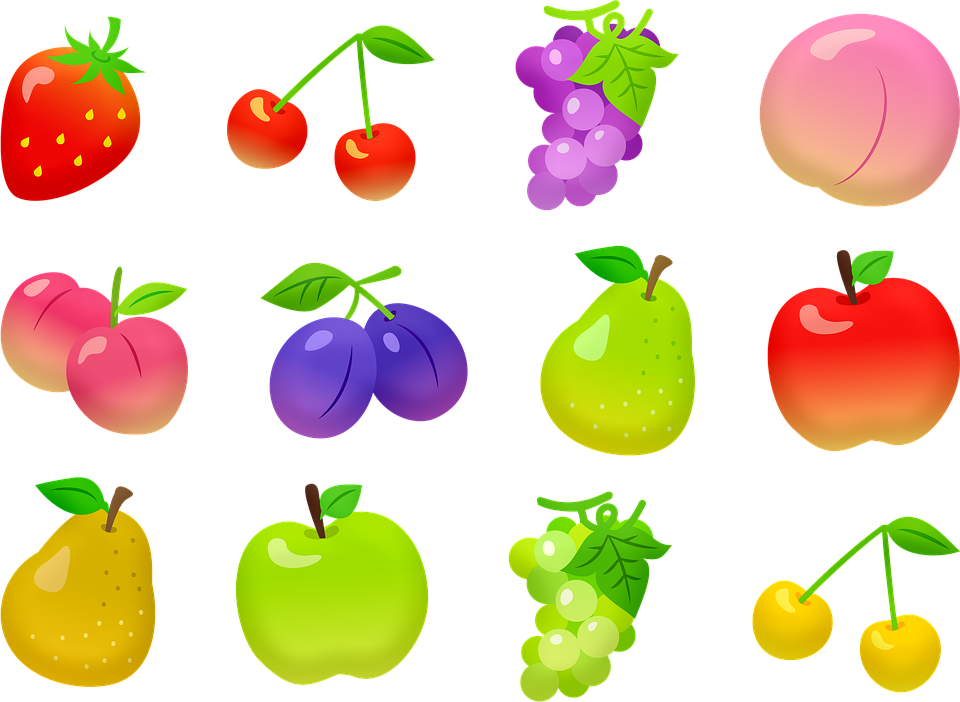
\includegraphics[trim=764 246 0 243, clip, width = 0.9cm]{02 - Combinatorics 101/fruits.png}};
            \node at (1.5 + 0.3*\x, 0 - 0.3*\x)
                {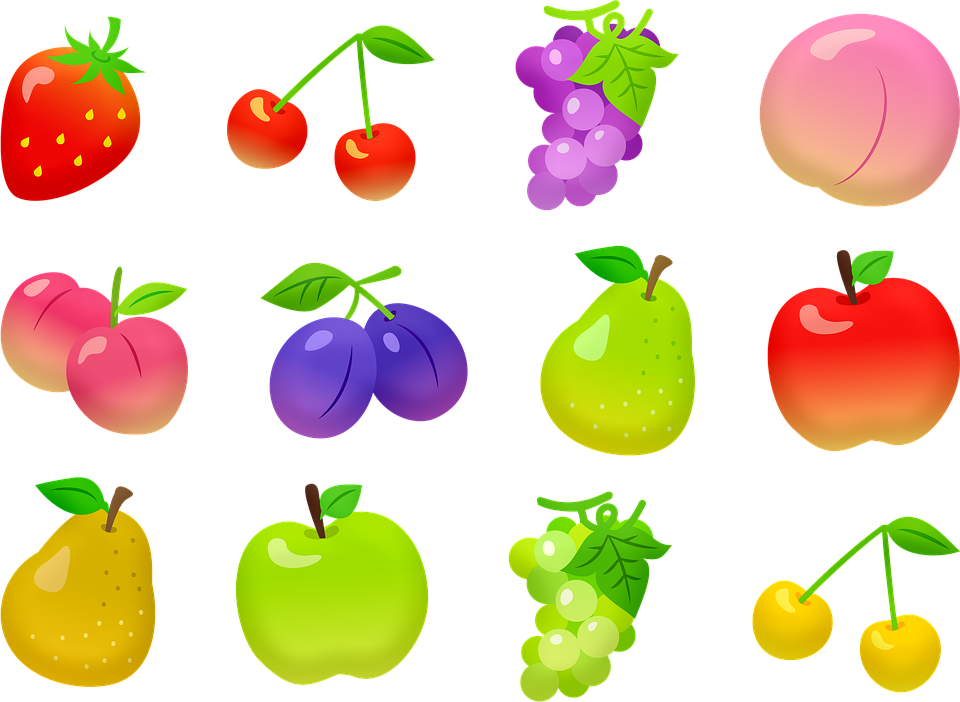
\includegraphics[trim=534 246 261 243, clip, width = 0.76cm]{02 - Combinatorics 101/fruits.png}};
            \node at (3 + 0.3*\x, 0 - 0.3*\x)
                {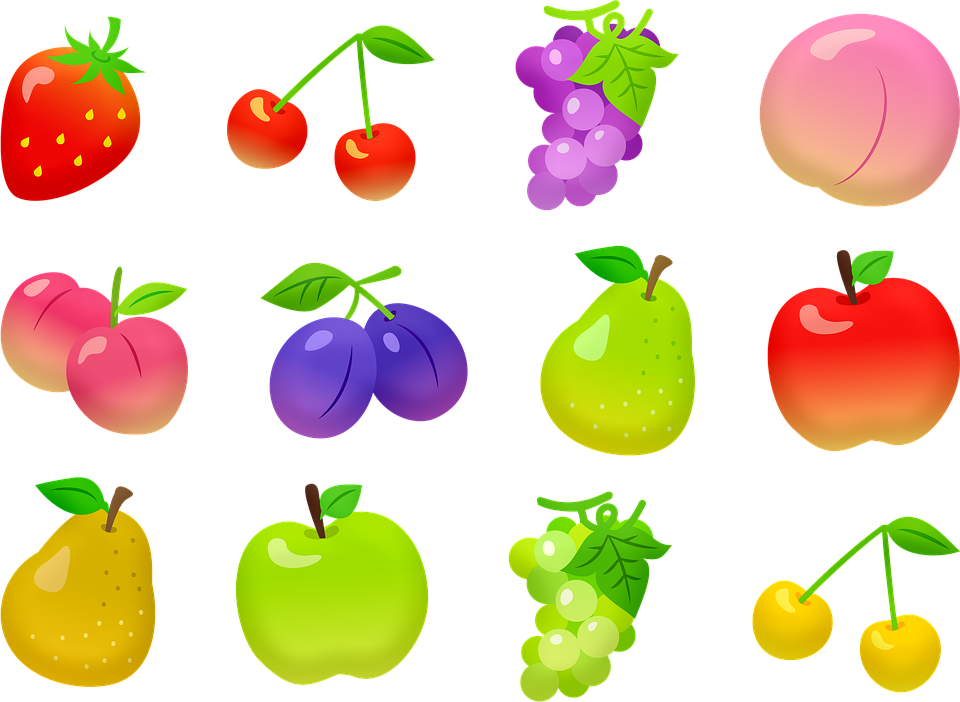
\includegraphics[trim=0 490 809 0, clip, width = 0.69cm]{02 - Combinatorics 101/fruits.png}};
            \node at (4.5 + 0.3*\x, 0 - 0.3*\x)
                {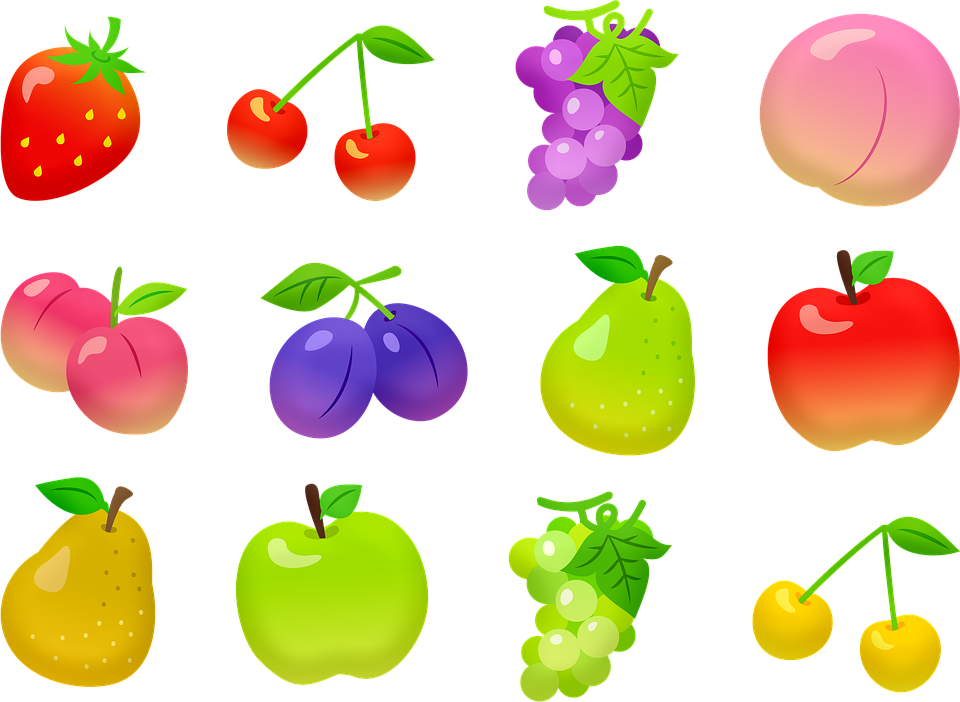
\includegraphics[trim=751 491 0 0, clip, width = 0.96cm]{02 - Combinatorics 101/fruits.png}};
          }
        \end{tikzpicture}
      \end{nscenter}

      Let’s consider the first fruit. We have $4$ options to choose from. For second fruit we also have the same $4$ options and so on. So, total numbers of ways is 
      \[
        \underbrace{4 \times 4 \times 4 \times 4 \times 4}_\text{$5$ times} = 4^5 = 1024.
      \]
    \end{column}
    \begin{column}{0.5\textwidth}
      \begin{definition}
        Sometimes permutations are not always about multiplication or division of factorials. Keep an eye on the exact wording of the problem and use the \emph{rules of sum}, \emph{product}, and \emph{division} with your best judgment.
      \end{definition}
    
      \begin{problem}
        {\color{textBlue} Example:} find number of divisors of $60$.
      \end{problem}

      {\small
      Let’s write $60$ as a product of prime numbers:
      \[ 60 = 2 \times 2 \times 3 \times 5 = 22 \times 31 \times 51.\]
      Any divisor of $60$ must be some combination of these prime numbers. Let’s count all combinations of prime factors of a divisor:

      The divisor may have $2$ in a power of $0$, $1$, or $2$ ($2$ to the power of $0$ is also counted, because divisor may be odd, like $15$, for example).

      The divisor may have $3$ in a power of $0$ or $1$.

      The divisor may have $5$ in a power of $0$ or $1$.

      So, total number of divisors of $60$ would be
      \[(2 + 1) (1 + 1) (1 + 1) = 12.\]
      }
    \end{column}
  \end{columns}
\end{frame}

\begin{frame}{Combinations}
  \begin{columns}[T]
    \begin{column}{0.5\textwidth}
      Let’s return back to fruits

      \begin{problem}
        There are $5$ different fruits on a plate: \emph{a red apple}, \emph{a pear}, \emph{a strawberry}, \emph{a peach}, and \emph{a green apple}. In how many ways can you take $3$ of them from the plate if \emph{order doesn’t matter}?
      \end{problem}

      \begin{nscenter}
        \begin{tikzpicture}[outer sep=0, inner sep=0, scale=1, transform shape]
          \node (apple1) at (0, 0)
              {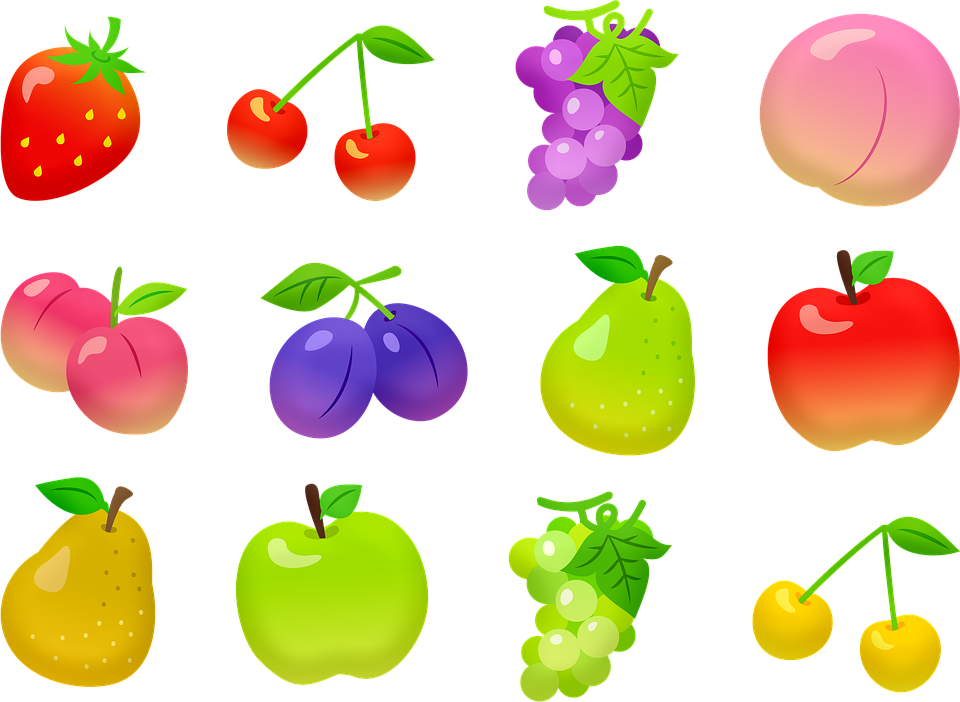
\includegraphics[trim=764 246 0 243, clip, width = 0.9cm]{02 - Combinatorics 101/fruits.png}};
          \node (pear1) at (1, 0)
              {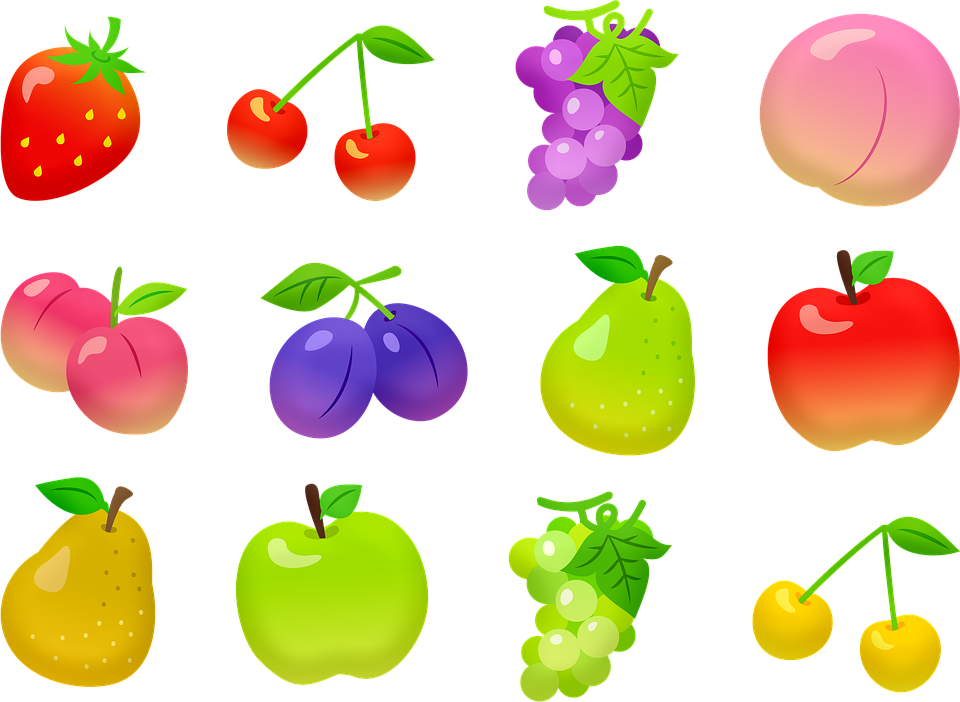
\includegraphics[trim=534 246 261 243, clip, width = 0.76cm]{02 - Combinatorics 101/fruits.png}};
          \node (strawberry1) at (1.95, 0)
              {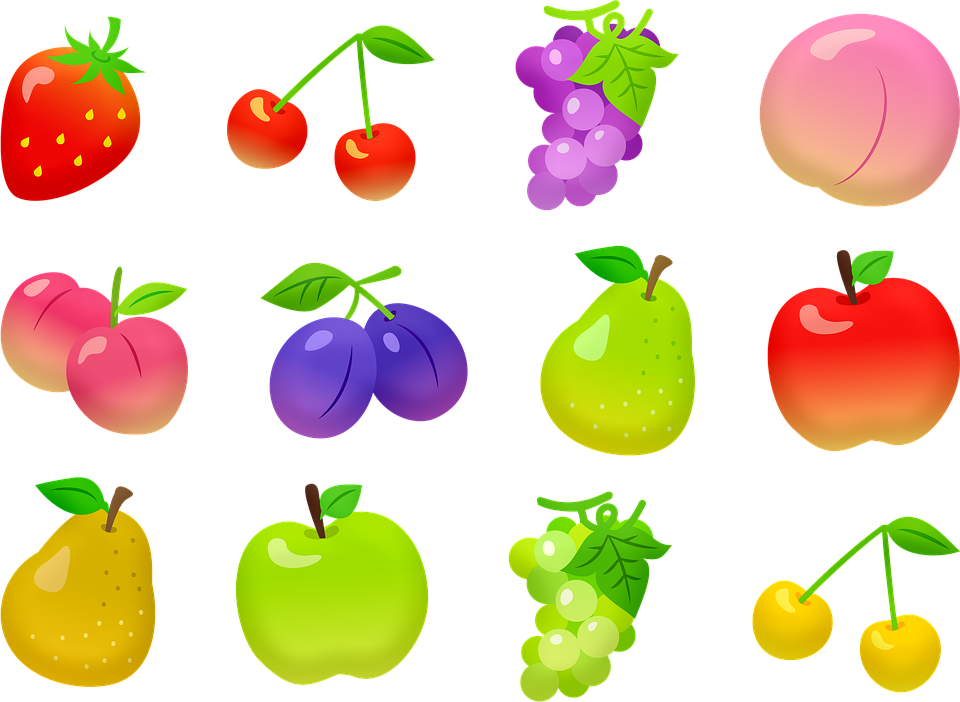
\includegraphics[trim=0 490 809 0, clip, width = 0.69cm]{02 - Combinatorics 101/fruits.png}};
          \node (peach1) at (2.9, 0)
              {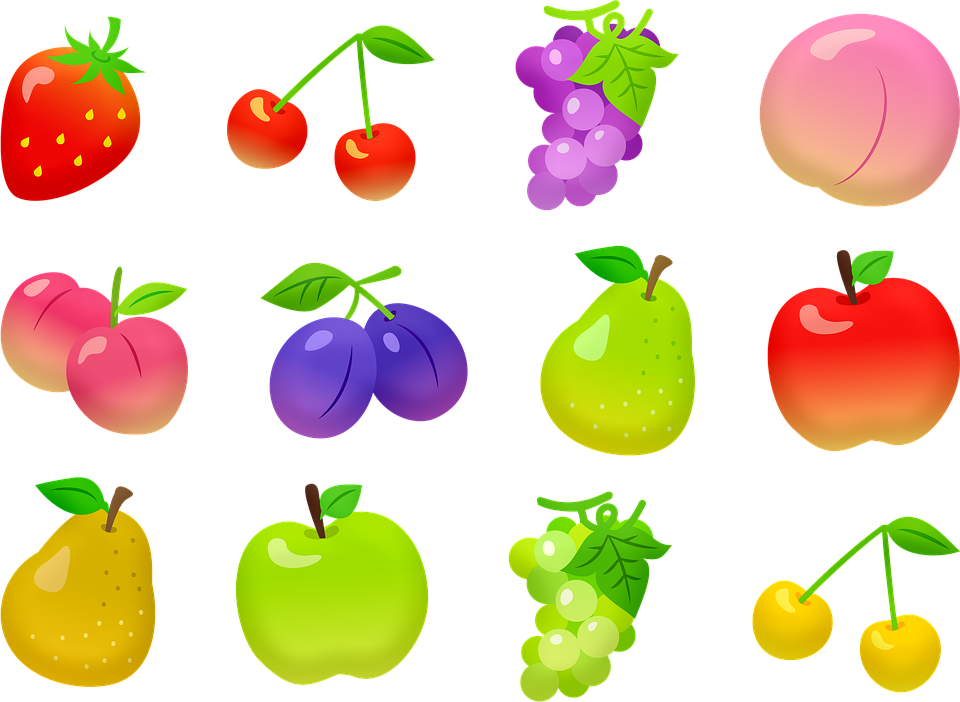
\includegraphics[trim=751 491 0 0, clip, width = 0.96cm]{02 - Combinatorics 101/fruits.png}};
          \node (apple2) at (4, 0)
              {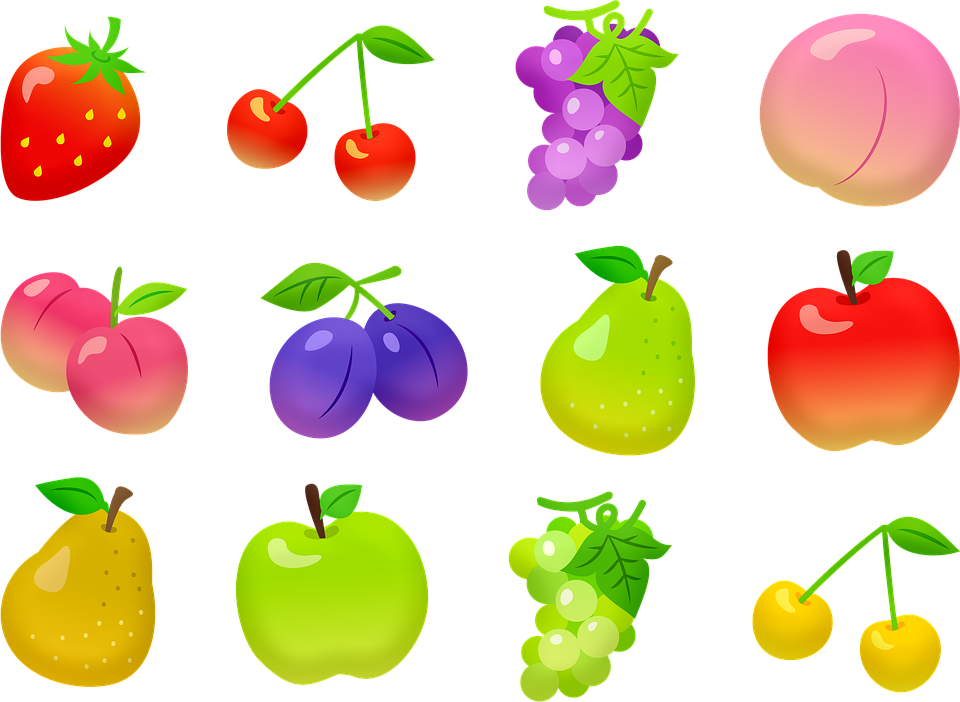
\includegraphics[trim=232 0 532 472, clip, width = 0.9cm]{02 - Combinatorics 101/fruits.png}};
        \end{tikzpicture}
      \end{nscenter}

      First, we know, that there are $P_3^5 = 5 \times 4 \times 3 = 60$ ways to select $3$ fruit \emph{one by one}, but in our case order is not important. So for every $3$ given fruits there are $3! = 6$ ways to select them them one by one. That means that each way to take $3$ fruits was counted $6$ times. As a result the total number of ways would be 
      \[
        \frac{5!}{2! \times 3!} = \frac{120}{2 \times 6} = 10.
      \]
    \end{column}
    \begin{column}{0.5\textwidth}
      \begin{definition}
        A \textbf{combination} is a way of choosing elements from a set in which order does not matter.
      \end{definition}

      To find a number of combinations of $k$ unordered elements from set of $n$ distinct objects (denoted as $C_k^n$ or $C(n,\ k)$), first we need to find $P_k^n$. Then, according the \emph{rule of division}, we need divide the number by number of ways to rearrange $k$ elements, which is $P_{\,k}$. Combining everything together we find, that
      \[
        C_k^n = \frac{n!}{k! (n-k)!}.
      \]
      The most common notation of the number of combinations is a \emph{binomial coefficient}:
      \[
        C_k^n = \binom{n}{k}.
      \]
      Reads: “\emph{$n$ choose $k$}”.

    \end{column}
  \end{columns}
\end{frame}

\begin{frame}{And beyond}
  \begin{columns}[T]
    \begin{column}{0.5\textwidth}
      Combinatorial problems may look similar, but you always need to be aware of specific conditions. Let's consider this set of problems.

      \begin{problem}%
        \begin{wrapfigure}[4]{r}{0.3\textwidth}%
          \vspace{-2em}
          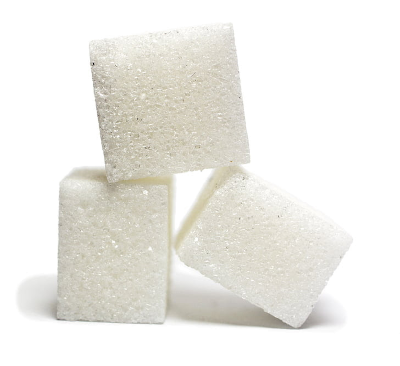
\includegraphics[width=0.3\textwidth]{02 - Combinatorics 101/sugar.png}
        \end{wrapfigure}

        There are $4$ sets of objects

        \quad $4$ \emph{cups} (all different),

        \quad $4$ \emph{glasses} (all the same),

        \quad $7$ \emph{teaspoons} (all different),

        \quad $10$ \emph{sugar cubes} (all the same).

        \begin{wrapfigure}[0]{r}{0.4\textwidth}%
          \vspace*{2em}
          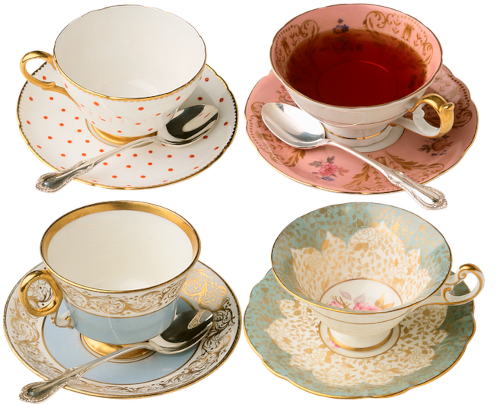
\includegraphics[width=0.45\textwidth]{02 - Combinatorics 101/cups.png}
        \end{wrapfigure}

        And we need to count the number of ways to put:

        \begin{enumerate}[a)]
          \item teaspoons into cups;
          \item sugar cubes into cups;
          \item teaspoons into glasses;
          \item sugar cubes into glasses.
        \end{enumerate}
      \end{problem}
      \begin{wrapfigure}[2]{r}{0.4\textwidth}\end{wrapfigure}
      Even though problems look the same, solutions are significantly different.
    \end{column}
    \begin{column}{0.5\textwidth}
      {\small
      Lets looks at the solutions:
      \begin{enumerate}[a)]
        \item This problem may be solved using \highlightbox{permutations with identical elements} (every spoon may be put in $4$ different cups), so answer is $4^7 = 16,384$.
        \item This problem may be solved using technique called \highlightbox{stars and bars}, (seen in a future lesson) calculated as $\binom{13}{3} = 286$.
        \item To calculate the solution we need to use \highlightbox{Stirling numbers of the second kind} and the \emph{rule of sum}:
        \[ {7\brace 1}+{7\brace 2}+{7\brace 3}+{7\brace 4}=1+63+301+350=715. \]\vspace*{-1ex}
        \item Here is we need to calculate number of \highlightbox{Young tableaux} with $10$ cells and $4$ boxes, which is far beyond middle school math. For this particular problem it is easier to just do the \highlightbox{\emph{\textbf{case}}\ \ \emph{\textbf{bashing}}} (head down and write out all cases) to find out that answer is $23$.  We’ll practice case bashing in a future lesson as well.
      \end{enumerate}
      }
    \end{column}
  \end{columns}
\end{frame}

\begin{frame}{Exercises}
  \begin{columns}[T]
    \begin{column}{0.5\textwidth}
      \begin{enumerate}
        \item Prove that $C^n_r$ is equal to $C^n_{n-r}$ using the formula in this unit. 
        
        \emph{Note that this is also can be proven logically, since if we are choosing $r$ out of $n$, we are equivalently not choosing $n-r$ out of $n$.}
        \item If $n = 100$, find the value of $\frac{(n−1)!}{(n+1)!}$.
        \item A yogurt shop has $4$ different flavours and $6$ different toppings. If a customer picks $1$ flavor and $2$ different toppings, how many different combinations are possible?
        \item How many $3$-digit numbers are palindromes (read the same forward and backward)?
        \item In base $7$, the possible digits are $0$-$6$. How many possible $4$-digit base $7$ numbers end in an odd digit?
        \seti
      \end{enumerate}
    \end{column}
    \begin{column}{0.5\textwidth}
      \begin{enumerate}
        \conti
        \item A ferris wheel has $8$ identical chairs that hold $1$ rider each. How many different ways can $8$ riders be seated on the ride, if we can only distinguish the relative orientation of the riders while the wheel is spinning?
        \item How many different $10$-letter code words can be made with the letters in Crittenden?
        \item How many $4$ digit ATM passcodes can be made if the first digit cannot be $0$, and all $4$ digits cannot be same?
      \end{enumerate}
      \begin{flushright}
        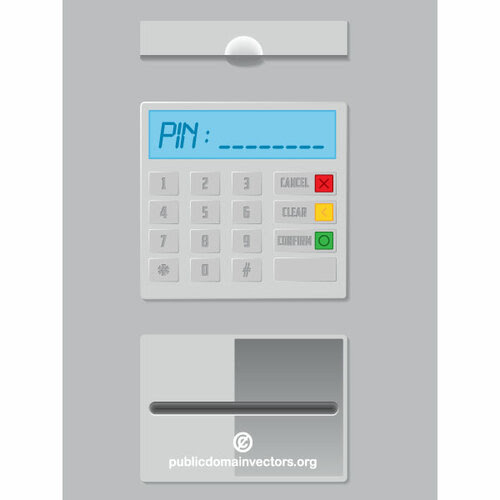
\includegraphics[width=0.4\textwidth]{02 - Combinatorics 101/atm.jpg}
      \end{flushright}
    \end{column}
  \end{columns}
\end{frame}

\begin{frame}{Challenge problems}
  \begin{columns}[T]
    \begin{column}{0.5\textwidth}
      \begin{enumerate}
        \item How many odd positive integers are factors of $480$?​
        \item A circular Beyblade has $5$ spots where decorative stickers can be placed around its edge. The Bey is otherwise perfectly symmetric circularly, so we can only distinguish a Bey by the relative orientation of the $5$ stickers.  If you must select $5$ unique stickers out of $10$ unique choices, how many distinguishable Beys can be created?​
        \item Two parents are taking their two children and $4$ of their friends to see a movie. They fill all of seats in an $8$-seat row. How many arrangements are possible if a parent must sit on each end on an aisle, and their two children must be seated next to one another?
        \seti
      \end{enumerate}
    \end{column}
    \begin{column}{0.5\textwidth}
      \begin{enumerate}
        \conti
        \item A game uses a deck of $n$ different cards, where $n \geq 6$. The number of possible set of $6$ cards that can be drawn from the deck is $6$ times the number of possible sets of $3$ cards that can be drawn from the deck. Find the value of $n$.
      \end{enumerate}
      \begin{center}
        \vspace*{1em}
        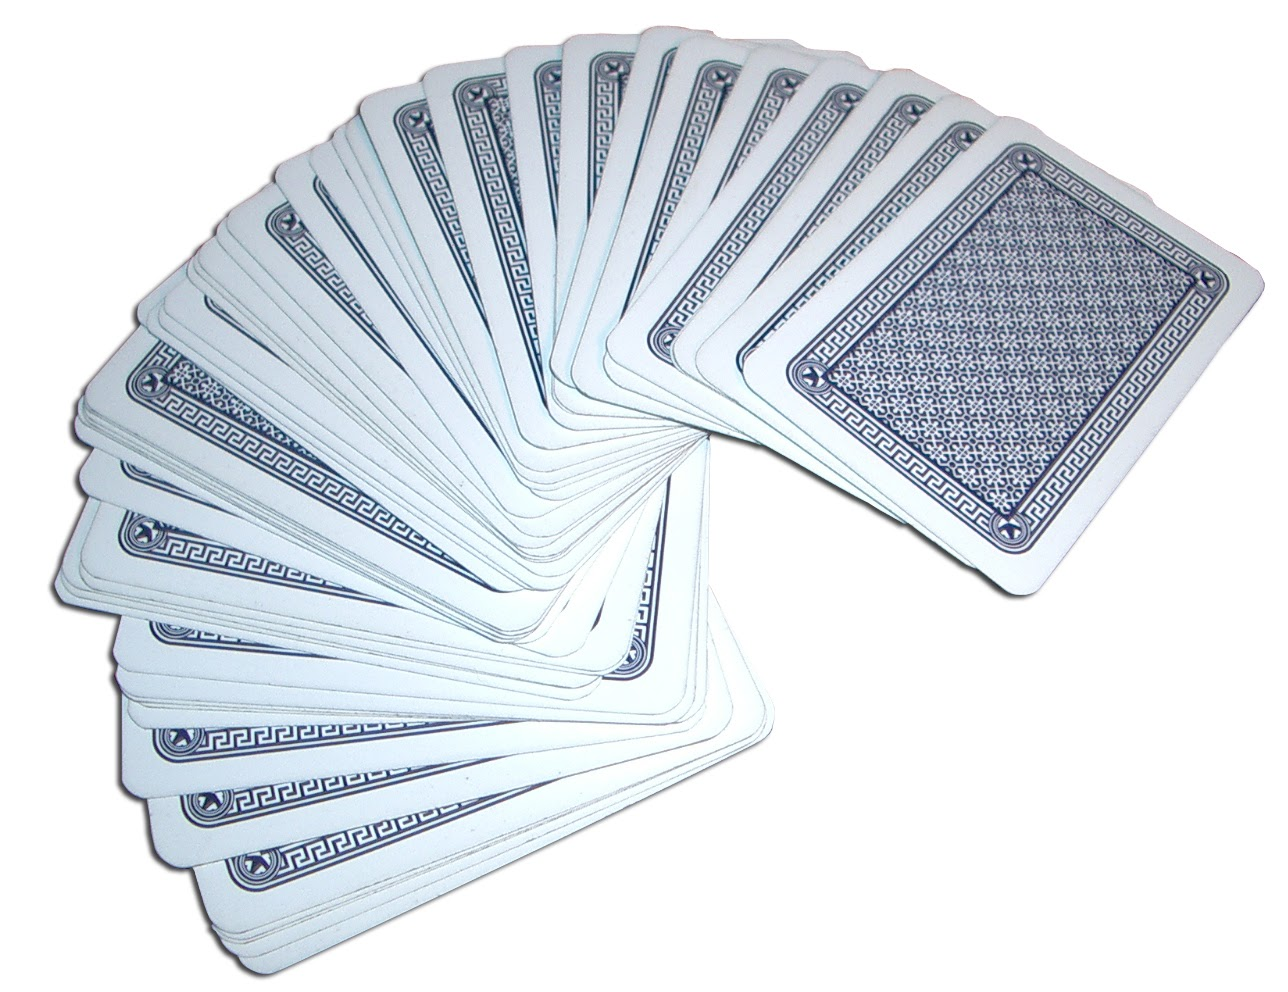
\includegraphics[width=0.8\textwidth]{02 - Combinatorics 101/cards.jpg}
      \end{center}
    \end{column}
  \end{columns}
\end{frame}

\begin{frame}{Team attack problems}
  \begin{columns}[T]
    \begin{column}{0.5\textwidth}
      \begin{enumerate}
        \item There are fewer than $50$ people at a party, and each person at the party shakes each other attendee’s hand once. If there are an odd number of total handshakes, what is the largest number of people there could be at the party?​
        \item King Arthur chose to have his knights in Camelot seated at a round table.  Including Arthur, there are $12$ people seated at the table.  If Arthur cannot be seated next to Lancelot, how many possible configurations are possible.  Note that only a change in relative position counts as a configuration.​
        \item A company with $4$ senior partners and $3$ junior partners wanted to form a $3$-person management committee with at least $2$ senior partners and at most $1$ junior partner.  How many different ways could they form this committee?
        \seti
      \end{enumerate}
    \end{column}
    \begin{column}{0.5\textwidth}
      \begin{enumerate}
        \conti
        \item What is the smallest number that has exactly $77$ divisors? You may use a calculator if that is helpful.​
        \item The coach of the Graham Math Olympiad Team wants to arrange their trophies in a single row in a display case.  If there are $3$ MOEMS trophies, $5$ Math League trophies, and $2$ Mathcounts trophies, how many ways can she arrange the trophies if the trophies for each type of contest must be kept together?​
        \item Two players are about to have a Pokemon card battle.  Each player has $10$ distinct cards, but can only select $6$ for the battle.  How many possible battle combinations are there for the match if the order of cards chosen does not matter?​
      \end{enumerate}
    \end{column}
  \end{columns}
\end{frame}

% \begin{frame}{Rule of product}
%   \begin{columns}[T]
%     \begin{column}{0.5\textwidth}
%     \end{column}
%     \begin{column}{0.5\textwidth}
%     \end{column}
%   \end{columns}
% \end{frame}
\end{document}
